\documentclass[a4paper,fleqn,12pt]{article}

\usepackage[utf8]{inputenc}
\usepackage[bulgarian]{babel}
\usepackage{amsmath}
\usepackage{amssymb}
\usepackage{booktabs}
\usepackage{fancyhdr}
\usepackage{amsthm}
\usepackage{graphicx}


\newtheorem{theorem}{Tеорема}[subsection]
\newtheorem{lemma}{Лема}[subsection]
\newtheorem{definition}{Дефиниция}[subsection]

\theoremstyle{definition}
\newtheorem{example}{Пример}[subsection]



\title{Математически анализ 2}
\author{Exonaut}

\pagestyle{fancy}
\fancyhf{}
\lhead{\rightmark}
\rhead{\thepage}
\cfoot{}
\renewcommand{\headrulewidth}{0pt}


\begin{document}

\pagenumbering{gobble}
\maketitle

\newpage
\pagenumbering{arabic}

\tableofcontents
\newpage

\section{Лекция 1: Пространството $\mathbb{R}^m$}

\subsection{Няколко важни неравенства}
Нека $a_k $ и $b_k (k = 1, 2, ..., m) $ са реални числа и $m \in \mathbb{N}$
\begin{theorem}[Неравенство на Коши-Шварц]
В сила е следното неравенство: \\
$$\left( \sum_{k=1}^{m}a_kb_k \right ) ^ 2   \leq  \left( \sum_{k=1}^{m}a_k \right)  \left( \sum_{k=1}^{m}b_k  \right) $$
\end{theorem}
Равенство се достига само когато $a_k$ и $b_k$ са пропорционални:\\
 ($\exists \lambda_0: b_k =\lambda_0 a_k  $)\\
Равенството може да се запише: 
$$\displaystyle\left\lvert \sum_{k=1}^{m}a_kb_k \right \rvert \leq \sqrt{\left( \sum_{k=1}^{m}a_k \right)}  \sqrt{ \left( \sum_{k=1}^{m}b_k  \right)} $$

\begin{theorem}[Неравенство на Минковски]
В сила е следното неравенство: \\
$$\sqrt{ \sum_{k=1}^{m} (a_k + b_k)^2}   \leq \sqrt{ \sum_{k=1}^{m}a_k^2 } + \sqrt{ \sum_{k=1}^{m}b_k^2 }$$
\end{theorem}
Равенство се достига само когато $a_k$ и $b_k$ са пропорционални.
Общ случай на неравенството на Минковски:
$$\left ( \sum_{k=1}^{m} \vert a_k + b_k\vert ^p \right)^\frac{1}{p}   \leq\left ( \sum_{k=1}^{m}\vert a_k\vert ^p\right)^\frac{1}{p} + \left ( \sum_{k=1}^{m} \vert b_k\vert ^p \right)^\frac{1}{p}   ( p\geq 1)$$

\begin{theorem}
В сила е следното неравенство: \\
$$ \vert a_k + b_k\vert   \leq \sqrt{ \sum_{k=1}^{m} (a_k + b_k)^2} \leq   \sum_{k=1}^{m}\vert a_k - b_k\vert  $$
\end{theorem}

\subsection{Видове крайно мерни пространства}

\subsubsection{Линейно(Векторно) пространство}
	\begin{definition}
Нека L е линейно(векторно) пространство над полето $R$. В него има въведени две операции: събиране и умножение на вектор с число.
		\begin{enumerate}
 			\item $x,y \in L \implies z = x+ y \in L $
			\item $x \in L, \lambda \in \mathbb{R} \implies z = \lambda x \in L$
		\end{enumerate}
\end{definition}

\subsubsection{Евклидово пространство}
\begin{definition}
Крайномерното пространство L се нарича евклидово, ако в него е въведено скаларно произведение, т.е за всеки два елемента $x,y \in L$ може да се съпостави реално число $(x,y)$, удовлетворяващо свойствата за линейност, симетричност и положителна определеност.
	\begin{enumerate}
 		\item $x,y,z \in L ,\lambda \in \mathbb{R} \implies (x+y,z) = (x,z) + (y,z); (\lambda x,y) = \lambda(x,y)$
		\item $x,y \in L \implies (x,y) = (y,x)$
		\item $x \in L, x\neq 0 \implies (x,x) > 0 $
	\end{enumerate}
\end{definition}

\subsubsection{Метрично пространство}
\begin{definition}
Крайномерното пространство L се нарича метрично, ако в него е въведено разстояние (метрика) $\rho$, т.е за два елемента $x,y \in L$ може да се съпостави неотрицателно число  $\rho \geq 0 $  със следните свойства
	\begin{enumerate}
 		\item $\rho(x,x) = 0 ; \rho(x,y) > 0 , x\neq y $
		\item $\rho(x,y) = \rho(y,x)$
		\item $\rho(x,z) \leq \rho(x,y) + \rho(y,z). \forall x,y,z \in L$
	\end{enumerate}
Метрично пространство L с метрика $\rho$ се означава $(L,\rho)$
\end{definition}

\subsubsection{Нормирано пространство}
\begin{definition}
Пространството се нарича нормирано, ако в него е въведена норма $\Vert. \Vert$, т.е $\Vert.\Vert: L \to \mathbb{R}_0^+$ със свойства 
	\begin{enumerate}
 		\item $x = 0  \implies \Vert x \Vert = 0, x \neq 0  \implies \Vert x\Vert > 0$
		\item $x \in L, \lambda \in \mathbb{R} \implies \Vert \lambda x \Vert = \vert \lambda\vert   \Vert x \Vert$
		\item $x,y \in L \implies \Vert x+y\Vert \leq \vert x\vert  + \vert y\vert $
	\end{enumerate}
\end{definition}
\begin{theorem}
Ако L е нормирано пространство с дадена норма $\Vert . \Vert$, то L е метрично пространство, т.е равенството $\rho(x,y) = \Vert x - y \Vert$ дефинира  разстоянието в L
\end{theorem}

\subsection{Пространството $\mathbb{R}^m$ - дефиниция и основни свойства}

\begin{definition}
Множеството от наредени m-торки $a = (a_1, a_2, ... , a_m)$ от реални числа. Числата $a_1, a_2, ... , a_m$ се наричат съответно първа, втора, ..., m-та кордината на а.\\
\\
 Ако имаме $a = (a_1, a_2, ... , a_m), b = (b_1, b_2, ... , b_m), ; \lambda \in \mathbb{R} $ то
	\begin{enumerate}
		\item $a+b =(a_1, a_2, ... , a_m) +  (b_1, b_2, ... , b_m) = (a_1 + b_1, a_2+b_2, ... , a_m + b_m) \in \mathbb{R}^m$
		\item $ \lambda a =(\lambda a_1,\lambda a_2, ... , \lambda a_m) \in \mathbb{R}^m $\\
	\end{enumerate}
\end{definition}

\subsubsection{Скаларно произведение}
Скаларно произведение се дефинира : $$ (a,b) = \left( \sum_{k=1}^{m}a_kb_k \right )$$\\
С така въведено скаларно произведение пространството $R^m$ се превръща в евклидово.

\subsubsection{Норма и метрика}
С равенството:
$$\Vert a\Vert := \sqrt{ \sum_{k=1}^{m}(a_k)^2  }$$ \\
се въвежда норма в $\mathbb{R}^m$.
\\
 Нормата генерира метрика в $\mathbb{R}^m$ с формула: 
$$\rho(a,b) := \Vert a-b\Vert = \sqrt{ \sum_{k=1}^{m} (a_k - b_k)^2} $$

\subsubsection{Скаларен квадрат}
Скаларен квадрат: $a^2 = (a,a) = \sum _{k=1}^{m}a_k^2$

\subsubsection{Неравенство на Коши-Шварц, чрез скаларен квадрат}
Коши-Шварц чрез скаларен квадрат: $(a,b)^2 \leq a^2b^2$ и $\vert (a,b)\vert \leq \Vert a \Vert \Vert b \Vert$

\subsubsection{Неравенство на Минковски, чрез скаларен квадрат}
Неравенство на Минковски чрез скаларен квадрат: $\Vert a+b \Vert\leq \Vert a \Vert + \Vert b \Vert$

\subsection{Точки и множества в $\mathbb{R}^m$}

\subsubsection{Паралелепипед}

\begin{definition}
Множеството\\
$$\Pi (a; \delta_1, \delta_2, ... ,\delta_m) = \{ x \in \mathbb{R}^m: -\delta_k < x_k -a_k < \delta_k   \}$$
се нарича отворен паралелепипед в $\mathbb{R}^m$ с център точката а.\\
\\
Множеството\\
$$\widetilde\Pi (a; \delta_1, \delta_2, ... ,\delta_m) = \{ x \in\mathbb{R}^m: -\delta_k \leq x_k -a_k \leq \delta_k   \}$$
се нарича затворен паралелепипед в $R^m$ с център точката а.\\
\\
Ако $\delta_1 = \delta_2 = ... = \delta_m = \delta$, получените множества $\Pi (a; \delta)$ и $\widetilde\Pi (a; \delta)$ се  наричат съответно отворен и затворен куб в $\mathbb{R}^m$ с център а.
 \end{definition}

\subsubsection{Сфера и кълбо}

\begin{definition}
Нека числото r > 0. Множеството \\
$$B(a;r) = \{ x \vert  x \in \mathbb{R}^m, \rho(x,a) <r \} = \{ x\vert  x \in \mathbb{R}^m, \Vert x-a \Vert < r \}$$\\
се нарича отворено кълбо в $\mathbb{R}^m$ с център a и радиус r, множеството \\
$$\widetilde B(a;r) = \{ x \vert  x \in \mathbb{R}^m, \rho(x,a) \leq r \} = \{ x\vert  x \in \mathbb{R}^m, \Vert x-a \Vert \leq r \}$$\\
се нарича затворено кълбо в $\mathbb{R}^m$ с център a и радиус r, а множеството \\
$$S(a;r) = \{ x \vert  x \in \mathbb{R}^m, \rho(x,a) = r \} = \{ x\vert  x \in \mathbb{R}^m, \Vert x-a \Vert = r \}$$\\
се нарича сфера в $\mathbb{R}^m$ с център a и радиус r, а множеството \\
\end{definition}

\begin{definition}
Точката а се нарича
\begin{itemize}
	\item вътрешна за множеството А, ако съществува отворено кълбо $B(a,\varepsilon): B(a,\varepsilon) \subset A$
	\item външна за А, ако съществува $B(a,\varepsilon): B(a,\varepsilon) \subset \mathbb{R}^m \setminus  A$
	\item контурна за А, ако за всяко $\varepsilon > 0: B(a,\varepsilon) \cap A \neq \varnothing $ и \\ $ B(a,\varepsilon) \cap (\mathbb{R}^m \setminus  A) \neq \varnothing$
	\item изолирана ако съществува $\varepsilon > 0: B(a,\varepsilon) \cap A = \{ a \}$
\end{itemize}
	
\end{definition}

\begin{definition}
Множеството $A \subset \mathbb{R}^m $ се нарича 

\begin{itemize}
	\item отворено, ако всяка негова точка е вътрешна 
	\item затворено, ако неговото допълнение  $\mathbb{R}^m \setminus A$ е отворено
\end{itemize}

\end{definition}

\begin{definition}
Околност на дадена точка $a \in \mathbb{R}^m $ се нарича всяко отворено множество, което я съдържа. Означава се с $U_a$.
\end{definition}

\begin{definition}
Точка а се нарича точка на сгъстяване на множеството $A \subset \mathbb{R}^m $, ако всяка нейна околност $U_a$ съдържа поне една точка на А, различна от а, т.е $U_a \cap (A\setminus \{ a \} \neq \varnothing $
\end{definition}

\begin{definition}
Величината \\
$$d = d(A) = \sup_{a',a'' \in A} \rho(a';a'')$$\\
се нарича диаметър на множеството  $A \subset \mathbb{R}^m $.
\end{definition}

\begin{definition}
Множеството  $A \subset \mathbb{R}^m $ се нарича ограничено, ако съшествува кълбо(с краен радиус), което го съдържа.
\end{definition}

\begin{definition}
Множеството  $A \subset \mathbb{R}^m $ се нарича компактно, ако А е затворено и ограничено.
\end{definition}

\begin{definition}
Множеството   $x = (x_1, x_2, ... , x_m) \in \mathbb{R}^m $, чийто кординати са непрекъснати функции $x_k = x_k(t) (k = 1, 2, ..., m)$, дефинирани върху даден интервал [a,b] се нарича непрекъсната крива в $R^m$. t се нарича параметър на кривата.\\
Точките $x(a) = (x_1(a), x_2(a), ... , x_m(a))$ и $x(b) = (x_1(b), x_2(b), ... , x_m(b))$ се наричат начало и край на дадената крива. Ако $x(a) = x(b)$ кривата е затворена
\end{definition}

\begin{definition}
Нека $x^0 = (x_1^0, x_2^0, ... , x_m^0) \in \mathbb{R}^m$ и $\alpha_1, \alpha_2, ... , \alpha_m$ са фиксирани числа за които $\sum_{k=1}^{m}\alpha_k > 0$. Множеството от точки $x = (x_1, x_2, ... , x_m)$ чиито кординати се представят във вида \\
$$x_k = x_k^0 + \alpha_kt, k = 1, 2, ..., m , -\infty < t <\infty $$\\
се нарича права линия в пространството $R^m$, минаваща през точка $x^0$ по направление $(\alpha_1, \alpha_2, ... , \alpha_m).$
\end{definition}

\begin{definition}
Множеството  $A \subset \mathbb{R}^m $ се нарича свързано,  ако за всеки две негови точки съществува непрекъсната крива $\gamma$, която ги свързва и $\gamma \subset A$.
\end{definition}

\begin{definition}
Множеството  $A \subset \mathbb{R}^m $ се нарича област, ако е отворено и свързано. Ако е и затворено, то се нарича затворена област. 
\end{definition}

\begin{definition}
Област, всеки две точки на която могат да се съединят с отсечка, изцяло лежаща в нея, се нарича изпъкнала област. 
\end{definition}

\begin{definition}
Областа $A \subset \mathbb{R}^m $ се нарича звездообразна област, отностно точката $x^0 \in A$, ако за вскяка точка $x \in A$ отсечката $[x^0,x]$ лежи изцяло в А. 
\end{definition}

\subsection{Редици от точки в $\mathbb{R}^m$}

\begin{definition}
Редицата $\{ x^{(n)} \}_{n = 1} ^ \infty = \{x_1 ^{(n)}, x_2 ^{(n)}, ... , x_m^{(n)}\} $ се нарича редица от точки в $\mathbb{R}^m$, а редицата $\{ x_k ^{(n)}\}_{n=1} ^ \infty ( k = 1 \div m) $ - к-та кординатна редица. За по кратко редицата $\{ x^{(n)} \}_{n = 1} ^ \infty$ се означава $\{ x^{(n)} \}$
\end{definition}

\begin{definition}
Редицата $\{ y^{(l)} \}_{l = 1} ^ \infty$ се нарича поредица на редицата $\{ x^{(n)} \}$ и се означава:\\
$\{ x^{(n_l)} \}, l = 1, 2, ..., $ или $\{ x^{(n_l)} \}_{l = 1} ^ \infty$\\
ако за всяко l съществува такова $n_l$, че $y^{(l)} = x^{(n_l)}$, при това, ако $l' < l'' $, то $n_{l'}<n_{l''}$.
\end{definition}

\begin{definition}
Редицата $\{ x^{(n)} \}$ се нарича сходяща към точка $a \in \mathbb{R}^m$ (граница на редицата), ако за всяко $\varepsilon > 0$ съществува такова $N_0 > 0$, че за всяко $n > N_0$ е изпълено неравенството $\rho(x^{(n)};a) = \Vert x^{(n)} - a \Vert < \varepsilon$. Ако редицата няма граница, се нарича разходяща. 
\end{definition}


\begin{definition}
Точката $a \in R^m$ се нарича точка на сгъстяване на редицата $\{ x^{(n)} \}$, ако всяка нейна околност съдържа безброй много членове на редицата. 
\end{definition}

\begin{theorem}
Нека $x^{(n)} \in \mathbb{R}^m$ за $n \in \mathbb{N} $ и точката $a \in \mathbb{R}^m$. Тогава 
$$(\{x^{(n)}\} \to a )\iff (x_k ^{(n)} \to a_k, k = 1 \div m)$$\\
T.e редицата има граница точката а, тогава и само тогава когато всяка от кординатите на редици $\{x_k^{(n)}\}$ има граница съответната кордината $a_k$ на точката а
\end{theorem}

\begin{theorem}[Критерий на Коши]
Нека $x^{(n)} \in \mathbb{R}^m$ за $n \in \mathbb{N} $. Редицата $x^{(n)}$ е сходяща тогава и само тогава когато за всяко $\varepsilon > 0$ съществува такова число $N_0 > 0$, че при всяко $n \in N, n > N_0$ и всяко $p \in \mathbb{N}$ е изпълено $\rho(x^{(n+p)}, x^{(n)}) = \Vert x^{(n+p)} - x^{(n)} \Vert < \varepsilon$
\end{theorem}

\begin{definition}
Редицата $\{x^{(n)}\}$ се нарича ограничена , ако съществува кълбо ( с краен радиус), което съдържа всичките ѝ членове. 
\end{definition}


\begin{theorem}[Болцано-Вайерщрас]
От всяка ограничена редица в пространството $R^m$ може да се избере сходяща подредица. 
\end{theorem}


\begin{definition}
Всяко множество $A \subset \mathbb{R}^m $ се нарича компактно, ако от всяка редица $\{x^{(n)}\}, x^{(n)} \in A$, може да се избере сходяща подредица $\{x_k ^{(n)}\}$ с граница принадлежаща на А
\end{definition}

\newpage

\section{Лекция 2: Функция на няколко променливи. Граница и непрекъснатост}

\subsection{Дефниция на функция на няколко променливи}

\begin{definition}
Казва се че дадена функция с дефиниционна област(дефиниционно множество) D, ако на всяка точка $x = (x_1, x_2, ... , x_m)$ от множеството D е съпоставено реално число $f(x) = f(x_1, x_2, ... , x_m)$, т.е на всяко $x \in D$ съществува единствено число $y = f(x) \in \mathbb{R}$. Понякога за кратко се записва. 
$$f: D \to \mathbb{R} $$\\
В $\mathbb{R}^2$ се използва $(x,y)$ за означение, а в $\mathbb{R}^3$ - $(x,y,z)$.
\end{definition}

\subsection{Граница на функция на няколко променливи}

\begin{definition}[Коши]
Нека $f: D \to \mathbb{R}, a \in \mathbb{R}^m$, а е точка на сгъстяване за D. Казва се че $f(x)$ има граница L при $x \to a$ със стойностти $x \neq a$ ако за всяко $\varepsilon > 0$ съществува $\delta > 0$, че за всяко x от множеството $D \setminus \{a\}$, за което $\rho(x;a) = \Vert x - a \Vert < \delta $ е изпълнено $\vert f(x) - L \vert  < \varepsilon$. Записва се $$\lim\limits_{x \to a} f(x) = L$$
\end{definition}

\begin{definition}[Хайне]
Нека $f: D \to\mathbb{R}, a \in \mathbb{R}^m$, а е точка на сгъстяване за D. Казва се че $f(x)$ има граница L при $x \to a$ със стойностти $x \neq a$ ако за всяка редица  $\{x^{(n)}\} ,x^{(n)} \in D, x^{(n)} \neq a$ сходяща към а, числовата редица $\{f(x^{(n)})\}$ има граница L. 
\end{definition}

\begin{theorem}
Дефинициите 2.2.1 и 2.2.2 на Коши и Хайне за граница на функция са еквивалентни.
\end{theorem}

\begin{definition}
Нека $f: D \to \mathbb{R}, a \in \mathbb{R}^m$, а е точка на сгъстяване за D. Казва се че $f(x)$ дивергира към $\infty$ (съответно към $-\infty$) при $x \to a$ със стойностти $x \neq a$, ако за всяко $A \in \mathbb{R}$ съществува такова $\delta > 0$, че за всяко x от множеството $D \setminus \{a\}$, за което $\rho(x;a) = \Vert x - a \Vert < \delta $ е изпълнено $f(x) > A $( съответно $f(x) < A)$. Записва се
 $$\lim\limits_{x \to a} f(x) = \infty (-\infty) $$ 
\end{definition}

\begin{definition}[Повторна граница]
Нека $D \subset \mathbb{R}^2, a = (a_1, a_2) \in \mathbb{R}^2$ e точка на сгъстяване за D и функция $f: D\to \mathbb{R}$. Нека съществува такава околност $U_{a_2} \subset \mathbb{R}$ на точката $а_2$, че за всички стойностти $y \in U_{a_2} $ да съществува  $\lim\limits_{x \to a_1} f(x,y) = \varphi (y)$. Ако освен това съществува $\lim\limits_{y \to a_2} \varphi (y) = A$, А се нарича повторна граница и се означава както следва 
$$A = A_{1,2} =\lim\limits_{y \to a_2} (\lim\limits_{x \to a_1} f(x,y) ) $$.\\
Аналогично се съвежда и другата повторна граница 
$$ A_{2,1} = \lim\limits_{x \to a_1} (\lim\limits_{y \to a_2} f(x,y) ) $$
\end{definition}

\begin{theorem}
Нека $D \subset \mathbb{R}^2, a = (a_1, a_2) \in \mathbb{R}^2$ e точка на сгъстяване за D и функция $f: D \to \mathbb{R}$.  Нека
\begin{enumerate}
		\item  Съществува такава околност $U_{a_2} \subset \mathbb{R}$ на точката $a_2$, че за всички стойностти $y \in U_{a_2} $ да съществува  $\lim\limits_{x \to a_1} f(x,y) = \varphi (y)$.

		\item Съществува границата $\lim\limits_{(x, y) \to (a_1,a_2) } f(x,y) = L$.
\end{enumerate}
Тогава съществува граница  $\lim\limits_{y \to a_2} \varphi (y)$ и освен това е в сила равенствотот  $\lim\limits_{y \to a_2} \varphi (y) = L$
\end{theorem}

\subsection{Непрекъснатост на функция на няколко променливи}

\begin{definition}
Казва се че функцията $f: D \to \mathbb{R}$ е непрекъсната в точка $a \in D$ ако $\lim\limits_{x \to a} f(x) = f(a)$.
\end{definition}

\begin{definition}[непрекъснатост по Коши]
Казва се, че функцията $f: D \to \mathbb{R}$ е непрекъсната в точка $a \in D$, ако за всяко $\varepsilon > 0$ съществува $\delta > 0$, че за всяко x от множеството $D $, за което $\rho(x;a) = \Vert x - a \Vert < \delta $ е изпълнено $\vert f(x) - f(a) \vert  < \varepsilon$.
\end{definition}

\begin{definition}[непрекъснатост по Хайне]
Казва се, че функцията $f: D \to \mathbb{R}$ е непрекъсната в точка $a \in D$ ако за всяка редица  $\{x^{(n)}\}$ (с $x^{(n)} \in D$ за $n \in \mathbb{N}$) сходяща към а, числовата редица $\{f(x^{(n)})\}$ има граница $f(a)$. 
\end{definition}

\begin{definition}[за съставна функция]
Нека $A \subset \mathbb{R}^m$ е отворено множество, $f: A \to \mathbb{R}$ и $x_k: (\alpha, \beta) \to \mathbb{R}, k = 1 \div m$. Полагайки  $x(t) = (x_1(t), x_2(t), ... , x_m(t)) \in A$ за всяко $t \in (\alpha, \beta)$ съставната функция $F(t) = f \circ x(t) = f(x(t))$ се дефинира по формулата 
$$F(t) = f \circ x(t) = f(x(t)) = f(x_1(t), x_2(t), ... , x_m(t))$$
\end{definition}

\begin{theorem}
Нека $A \subset \mathbb{R}^m$ е отворено множество и $f: A \to \mathbb{R}$ интервалът $(\alpha, \beta) \subset \mathbb{R}$ , $x_k: (\alpha, \beta) \to \mathbb{R} $ за $k = 1 \div m$. Нека освен това $x(t) = (x_1(t), x_2(t), ... , x_m(t)) \in A$ за $\forall t \in (\alpha, \beta)$ и $x_k$ са непрекъснати в точката $t_0 \in (\alpha, \beta) $  за $k = 1 \div m$, а $f$ e непрекъсната в $x^0 = x(t_0)$. Toгава функцията $F(t) = f \circ x(t) = f(x(t)) = f(x_1(t), x_2(t), ... , x_m(t))$ е непрекъсната в точката $t_0$
\end{theorem}

\subsection{Равномерна непрекъснатост на функция на няколко променливи}
\begin{definition}
Нека $A \subset \mathbb{R}^m$ е отворено множество и $f: A \to \mathbb{R}$. Функцията се нарича равномерно непрекъсната в A, ако за  всяко $\varepsilon > 0$ съществува $\delta = \delta(\epsilon)$, че за всеки две точки $x', x'' \in A$ за които разстоянието $\rho(x';x'') =\Vert x' - x'' \Vert < \delta $, да следва, че $\vert f(x') - f(x'') \vert  < \varepsilon$.
\end{definition}

\begin{theorem}[на Вайерщрас]
Нека множеството $K \subset \mathbb{R}^m$ е компактно и функцията $f: K \to \mathbb{R}$ е непрекъсната върху K. Tогава 

\begin{enumerate}
		\item f е ограничена в К, т.е същестуват $m, M \in \mathbb{R}$ такива че за всички $x \in K$ е изпълнено неравенството
$m \leq f(x) \leq M$
		\item f достифа най малката и най-голямата си стойност в К, т.е съществуват точки $x^0, y^0 \in K$ , такива че
$$f(x^0) = \inf _{x \in K}f(x) ; f(y^0) = \sup_{y \in K} f(x)$$
\end{enumerate}

\end{theorem}

\begin{theorem}[на Kантор]
Нека множеството $K \subset \mathbb{R}^m$ е компактно и функцията $f: K \to \mathbb{R}$ е непрекъсната върху K. Тогава $f$ е равномерно непрекъсната върху K.
\end{theorem}


\newpage

\section{Лекция 3: Частни производни. Диференцируемост на функция на две и повече променливи}
 
\subsection{Дефиниция на частна производна}
Ще дефинираме елементи които ще се използват. 
\begin{itemize}
	\item $D \subset \mathbb{R}^m$ -  отворено множество
	\item $x^0 = (x_1 ^ 0, x_2 ^ 0, ... , x_m ^ 0)$ - точка, принадлежаща на D
	\item $U_{x^0} \subset D$ - околност на $x^0$
	\item $U_{x_i ^ 0} \subset D$ - oколност на $x_i ^ 0$ (i  = 1, 2, ..., m)
	\item точката $(x_1 ^ 0, x_2 ^ 0, ..., x_{i-1}^0, x_i ^ 0, x_{i+1} ^i, ..., x_m ^ 0) \in U_{x^0}$, за всички стойности на $x_i \in U_{x_i ^ 0}$
	\item $f$ и $g$ - функции, дефинирани съответно в $D$ и $U_{x_i ^ 0}$. т.е \\
$f: D \to \mathbb{R} , g: U_{x_i ^ 0} \to \mathbb{R}$ и $g(x_i) = f(x_1 ^ 0, x_2 ^ 0, ..., x_{i-1}^0, x_i ^ 0, x_{i+1} ^i, ..., x_m ^ 0)$
\end{itemize}
 
\begin{definition}
Производната, ако съществува на функцията $g$ в точката $x_i ^ 0$ се нарича частна производна на функцията f( по променлива  $x_i ^ 0$) в точката $x^0$. Използва се означението $\dfrac {\partial f(x^0)}{\partial x_i}$ или $f'_{x_i} (x^0)$. \\
Частната производна на функцията $f$ отностно променливата $x_i$ е равна на границата на функцията $\varphi (h_i)  = \dfrac{g(x_i ^0 + h_i) - g(x_i ^ 0)}{h_i}$ при $h_i \to 0$ (ако съществува) т.е
$$\lim_{h_i \to 0} \varphi (h_i) = \lim_{h_i \to 0} \dfrac{g(x_i ^0 + h_i) - g(x_i ^ 0)}{h_i} = \dfrac {\partial f(x^0)}{\partial x_i}$$
\end{definition}

\begin{example}
\begin{gather*}
f(x,y) = x^2 + 9xy^2\\
f'_x (x,y) = (x^2)'_x+(9xy^2)'_x = 2x + 9y^2\\
f'_y (x,y) = (x^2)'_y+(9xy^2)'_y = 0 + 9x \cdot 2 \cdot y = 18xy \\
\end{gather*}
\end{example}

\subsection{Частни производни от по-висок ред}

\begin{definition}
Частната производна на частната производна от $n-1$ ред, $n = 1, 2, ...$(aко съществува), се нарича частична производна от $n$-ти ред. Частните производни, получени при диференциране по различни променливи се наричат смесени производни, а получените при диференциране само по една и съща променлива се наричат чисти производни. 
\end{definition}

\begin{example}
\begin{gather*}
f(x,y) = x^3\sin(6y) + x^2y^3 + 2222, f''_{x,y} = ?, f''_{y,x} = ? \\
\\
f''_{x,y} = (f'_x(x,y))'_y\\
f'_x(x,y) =(x^3\sin(6y))'_x + (x^2y^3)'_x + (2222)'_x = 3x^2 \sin(6y) + 2xy^3 + 0 \\
f''_{x,y} = (3x^2 \sin(6y) + 2xy^3)'_y \\
f''_{x,y} = (3x^2 \sin(6y))'_y + (2xy^3)'_y  =3x^2 \cos(6y).6 + 2.3xy^2 = 18x^2\cos(6y) + 6xy^2\\
\\
f''_{y,x} = (f'_y(x,y))'_x\\
f'_y (x,y) =(x^3\sin(6y))'_y + (x^2y^3)'_y + (2222)'_y \\
f'_y (x,y) = x^3 \cos(6y).6 + x^2.3y^2 + 0 = 6x^3 \cos(6y) + 3x^2y^2 \\
f''_{y,x} = (6x^3 \cos(6y) + 3x^2y^2)'_y = (6x^3 \cos(6y))_y + (3x^2y^2)'_y \\
f''_{y,x} = 6.3.x^2 \cos(6y) + 3.2.xy^2 = 18x^2\cos(6y) + 6xy^2 \\
\end{gather*}
\end{example}

\begin{theorem}[за равенство на смесени производни]
Нека точката $(x_0, y_0) \in \mathbb{R}^2$ и нека функцията $f$ е дефинирана в отвореното множество $U=U_{(x_0, y_0)} \subset \mathbb{R}^2$, което е нейната област т.е $f: U \to \mathbb{R}$. Нека освен това съществуват частните производни $f'_x, f'_y,f''_{x,y},f''_{y,x}$ за всички $(x, y)\in U$ и $f''_{x,y},f''_{y,x}$ са непрекъснати в точката $(x_0, y_0)$. Тогава е изпълнено равенството 
$$f''_{x,y}(x_0, y_0) = f''_{y,x}(x_0, y_0)$$
\end{theorem}

\subsection{Диференцируемост на функция}
Ще дефинираме елементи които ще се използват. 
\begin{itemize}
	\item $x^0 \in \mathbb{R}^m$
	\item $U \subset \mathbb{R}^m$ - отворено множество, което е околност на $x^0$.Без ограничение на общността може да се счита че U e $\delta$-околност на $x^0$ т.е U е отворено кълбо $B(x^0;\delta)$ с център $x^0$ и радиус $\delta$
	\item $f: U \to \mathbb{R}$ - функция дефинирана в $U = B(x^0;\delta) $
\end{itemize}

\begin{definition}
Функцията $f$ се нарича диференцируема в точка $x^0$ ако съществуват числа $A_1, A_2, ..., A_m$ и функция $\varepsilon (x^0, x - x^0)$, дефинирана за всички допустими стойности на $x \in U$ и $x - x^0 = (x_1 - x_1 ^0, x_2 - x_2 ^0,... x_m - x_m ^0)$, като при това 
$$f(x) - f(x^0) = \sum_{k=1}^{m} A_k(x_k + x_k ^ 0) + \varepsilon (x^0, x - x^0) \Vert x - x^0 \Vert$$ 
и $\lim\limits_{\Vert x - x^0 \Vert \to 0}\varepsilon (x^0, x - x^0) = 0$
\end{definition}

\begin{definition}
Функцията $f$ се нарича диференцируема в отвореното множество $U$, ако тя е диференцируема във всяка негова точка. 
\end{definition}

\begin{theorem}
Ако функцията $f: U \to \mathbb{R}$ е диференцируема в точката $x^0 \in U$, то тя е непрекъсната. 
\end{theorem}

\begin{definition}
В случай на диференцируемост в точката $x^0$ на функцията $f: U \to \mathbb{R}$, изразът 
$$df(x^0) \circ (h) = A_1 h_1 + A_2 h_2 + ... + A_m h_m$$
(или $df, df(x^0)$) се нарича пълен диференциал на $f(x)$ в точката $x^0$
\end{definition}

\begin{theorem}
Ако функцията $f: U \to \mathbb{R}$ е диференцируема в точката $x^0 \in U$, то съществуват частните производни $\dfrac{\partial f(x^0)}{\partial x_k}$ в точката $x^0$ и освен това $A_k(x^0) = \dfrac{\partial f(x^0)}{\partial x_k}, k = 1 \div m$.
\end{theorem}

\begin{definition}
Ако функцията $f: U \to \mathbb{R}$ е диференцируема в точката $x^0 \in U$, то със следната формула се изразява нейната производна в точката $x^0$
$$f'(x^0) = (f'_{x_1}(x^0), f'_{x_2}(x^0), ..., f'_{x_m}(x^0))$$.

\end{definition}

\begin{theorem}
Ако функцията $f: U \to \mathbb{R}$ притежава частни производни $\dfrac{\partial f(x^0)}{\partial x_k}, k = 1 \div m$ в отвореното множество U и освен това са непрекъснати в точката $x^0 \in U$, то $f$ е диференцируема в точката $x^0$.
\end{theorem}

\begin{definition}
Ако функцията $f: U \to \mathbb{R}$ притежава частни производни в U и тези частични производни са непрекъснати в точката $x^0 \in U$, то функцията се нарича непрекъснато диференцируема в точката $x^0$. Ако тези производни са непрекъснати в U, то функцията се нарича непрекъсанот диференцируема в това множество. 
\end{definition}

\begin{definition}
Диференциалът на диференциала от $n-1$ ред (n = 2, 3, ...) от функцията f(ако съществува) се нарича диференциал от n-ти ред(n-ти диференциал) на тази функция и се бележи $d^n f$\\
\\
Ако f е два пъти непрекъсната и диференцируема в $x^0 \in U$ тогава втория диференциал получава по следния резултат
$$d^2 f(x^0) = \sum_{i=1}^ m \sum_{j=1}^m f''_{x_i x_j}(x^0) dx_i dx_j = \left( \dfrac{\partial}{\partial x_1}dx_1 + ... + \dfrac{\partial}{\partial x_m}dx_m\right )^2 f(x^0)$$
което е симетрична квадратична форма на $dx_i (i = 1 \div m)$. \\
\\
Aналогично ако f е n пъти непрекъсната и диференцируема в $x^0 \in U$, то $d^n f(x^0)$ съществува и се дава със следната формула 
$$d^n f(x^0) = \left( \dfrac{\partial}{\partial x_1}dx_1 + ... + \dfrac{\partial}{\partial x_m}dx_m\right )^n f(x^0)$$
\end{definition}

\newpage

\section{Лекция 4: Диференциране на съставна функция. Производна по посока. Градиент. Допирателна. Нормална права}

\subsection{Диференциране на съставна функция}
$x^0 \in \mathbb{R}^m$ и отворено множество $U \subset \mathbb{R}^m$ е околност на точката $x^0$ (Без ограничение на общността може да се счита че U e $\delta$-околност на $x^0$ т.е U е отворено кълбо $B(x^0;\delta)$ с център $x^0$ и радиус $\delta$). \\
$t_0 \in (\alpha, \beta) \subset R$

\begin{theorem}
Нека функцията $f$ e дефинирана в U, а $\varphi_k$ - в интервала $(\alpha, \beta)$, т.е \\
$f: U \to \mathbb{R}$ и $\varphi_k: (\alpha, \beta)  \to \mathbb{R} $ $ (k = 1 \div m)$\\
като при това $x_k = \varphi_k(t)$ за $ k = 1 \div m $, $ \varphi_1(t),  \varphi_2(t), ...,  \varphi_m(t) \in U$ за всички стойности на $t \in (\alpha, \beta)$. Нека $f$ е диференцируема в U, $f'_k$ са непрекъснати в $x^0$ за $ k = 1 \div m$, $\varphi_k$ са диференцируеми в $t_0$ и $F: (\alpha, \beta)  \to \mathbb{R}$ е дефинирана с равенствово. \\
$$F(t) = f(\varphi_1(t),  \varphi_2(t), ...,  \varphi_m(t)), t \in (\alpha, \beta)$$
Тогава функцията F е диференцируема в $t_0$ и в сила е следното равенство
$$F'(t_0) = \sum_{k =1}^m f'_{x_k}(x^0)\varphi '_k (t_0)$$ \\
За m = 2: \\
$\varphi_1(t) = \varphi(t) , \varphi_2(t) =\psi(t) $
$$F'(t_0) = f'_x(x_0, y_0)\varphi'(t_0) + f'_y(x_0, y_0)\psi'(t_0)$$
\end{theorem}

\begin{example}
$f(x,y)$ - дефинирана и диференцируема в $U_{(1,2)} \subset \mathbb{R}^2$. с непрекъснати частни производни $f'_x, f'_y$ в точката (1,2). \\
Намерете производната $F'(0)$ на съставната фунция F, зададена с равенството $F(t) = f(1+3t, 2+4t)$.
\begin{gather*}
t_0 = 0 \\
x = \varphi(t) = 1+3t \\
y = \psi(t) = 2 + 4t \\
x_0 = \varphi(0) = 1 \\
y_0 = \psi(0) = 2 \\
\varphi'(t) = 3 \\
\psi'(t) = 4 \\
F'(t_0) = f'_x(x_0, y_0)\varphi'(t_0) + f'_y(x_0, y_0)\psi'(t_0) \implies  F'(0) = 3f'_x(1,2) + 4f'_y(1,2)
\end{gather*}
\end{example}

\subsection{Производна по посока. Градиент}
Нека $x^0 \in \mathbb{R}^m$ и лъчът $l$ е дефиниран, както следва: $$l:x = x^0 + t\nu, t > 0$$
Функцията f е дефинирана върху този лъч, а $$\varphi(t) := f(x(t)) = f(x^0 + t\nu), t > 0$$

\begin{definition}
Границата(ако съществува) 
$$\lim\limits_{t \to 0, t > 0} \dfrac{\varphi(t) - \varphi(0)}{t} = \lim\limits_{t \to 0, t > 0} \dfrac{\varphi(x^0 + t\nu) - \varphi(x^0)}{t} $$
се нарича производна на $f$ в точката $x^0$ по посока на вектора $\nu$ и се означава $\dfrac{\partial f(x^0)}{\partial \nu}$, т.е
$$\dfrac{\partial f(x^0)}{\partial \nu} = \lim\limits_{t \to 0, t > 0} \dfrac{\varphi(t) - \varphi(0)}{t} = \lim\limits_{t \to 0, t > 0} \dfrac{\varphi(x^0 + t\nu) - \varphi(x^0)}{t}$$ ако същестува границата.\\
\\
Ако частните производни съществуват, са производни "по посока на кординатните оси". \\
\\
Ако $f$ е дефинирана и диференцируема в околността $U_{x^0}$ на точката в $x^0$ и $f'_{x_k}$ са непрекъснати в $x_0$, то съществува производната ѝ по посока на вектора $\nu = (\nu_1, \nu_2, ..., \nu_m)$ и 
$$\dfrac{\partial f(x^0)}{\partial \nu} = \sum_{k = 1} ^m \nu_k \dfrac{\partial f(x^0)}{\partial x_k}$$
\end{definition}

\begin{definition}
Векторът с кординати $f'_{x_1}(x^0), f'_{x_2}(x^0), ..., f'_{x_m}(x^0)$ се нарича градиент на $f$ в точката $x^0$ и се означава 
$$grad \, f(x^0) = (f'_{x_1}(x^0), f'_{x_2}(x^0), ..., f'_{x_m}(x^0))$$
Предвид тази дефиниция, формулата за производна по посока на вектор $\nu$ се записва по кратко във вида
$$\dfrac{\partial f(x^0)}{\partial \nu} = grad \, (f(x^0), \nu)$$
\end{definition}

\begin {theorem}
Ако функцията $f$ е дефинирана и диференцируема в околността $U_{x^0}$ на точката в $x^0$ и $f'_{x_k}$ са непрекъснати в $x_0$, то съществува производната на $f$ по посока на  произволен вектора $\nu = (\nu_1, \nu_2, ..., \nu_m)$ и тя се дава с формула: $\dfrac{\partial f(x^0)}{\partial \nu} = grad \, f(x^0)$
\end {theorem}
Ако, $\nu$ е единичен вектор, т.е $\Vert \nu \Vert = 1$. \\
Тогава е в сила неравнестово $\left \vert  \dfrac{\partial f(x^0)}{\partial \nu}\right\vert  \leq \Vert grad \, f(x^0)  \Vert$, което следва от неравенство на Коши. 
$$\left \vert  \dfrac{\partial f(x^0)}{\partial \nu}\right\vert  = \left\vert  grad \, (f(x^0), \nu) \right\vert  \leq \Vert grad \, f(x^0) \Vert \Vert \nu \Vert = \Vert grad \, f(x^0)  \Vert$$
Равенство се достига само когато $\nu$ и $f(x^0)$ са колинеарни (еднопосочни или успоредни). тогава
$$\left \vert  \dfrac{\partial f(x^0)}{\partial \nu}\right\vert  = \Vert grad \, f(x^0)  \Vert$$
\\
Ако вектора $\nu$ е колинеарен с градиента, тогава векторът $\nu =  \dfrac{grad \, f(x^0)}{\Vert grad \, f(x^0) \Vert}$ и тогава 
$$
\dfrac{\partial f(x^0)}{\partial \nu} = \left( grad \, f(x^0),  \dfrac{grad \, f(x^0)}{\Vert grad \, f(x^0) \Vert} \right) = \Vert grad \, f(x^0) \Vert
$$
Ако $grad \, f(x^0) \neq 0$ то производната достига най голяма стойност единствено, ако диференцирането се извършва по посока на градиента. С други думи, посоката на градиента е посоката на най бързо нарастване на функцията, а големината му е равна на производната по тази посока. \\
\\
Ако $\nu = (\cos \alpha_1, \cos \alpha_2, ..., \cos \alpha_m)$, то производната по посока $\nu$ става 
$$\dfrac{\partial f(x^0)}{\partial \nu} = f'_{x_1}(x^0)\cos{\alpha_1} + f'_{x_2}(x^0)\cos{\alpha_2} + ... + f'_{x_m}(x^0)\cos{\alpha_m}.$$

\subsection{Допирателна равнина. Нормална права}

\begin{itemize}
\item $(x_0, y_0) \in \mathbb{R}^2$ - точка в $\mathbb{R}^2$
\item $M_0 (x_0, y_0, z_0) \in \mathbb{R}^3$  точка в $\mathbb{R}^3$
\item $U = U_{(x_0,y_0)} \subset \mathbb{R}^2 =$ - околност на $(x_0,y_0)$ 
\item $f: U \to \mathbb{R}$ - функция 
\item $z_0 = f(x,y)$ 
\item $S: z = f(x,y) \iff  S: f(x,y) - z = 0$ - уравнение на равнина 
\item $f'_x, f'_y$ - първи частни производни за всички $(x, y) \in U$,$ f'_x, f'_y$ са непрекъснати в точката $(x_0, y_0)$
\end{itemize}

\begin{definition}
Равнината $\tau (\tau \nparallel Oz)$, зададена с уравнение 
$$\tau : z - z_0 = f'_x (x_0, y_0)(x - x_0) + f'_y (x_0, y_0)(y - y_0) $$
се нарича допирателна (тангенциална) равнина в точкат $M_0$ към повърхнината S и представлява графиката на $f(x,y)$. 
\end{definition}

\begin{definition}
Векторите $n_1, n_2$
$$n_1 (-f'_x (x_0, y_0), -f'_y (x_0, y_0), 1) \qquad n_2 (f'_x (x_0, y_0), f'_y (x_0, y_0), -1) ,$$ 
които са нормални вектори на тангенциалната равнина, се наричат нормални вектори и за повърхнината S. \\
$n_1 = -n_2$ Това позволява да се използват за ориентация на повърхината S. \\
Горната страна се дефинира с вектора $n_1$ за който ъгъл $\measuredangle (n_1,k)$ е остър. 
\end{definition}

\begin{definition}
Правата n, зададена с уравнение 
$$n: \dfrac{x - x_0}{-f'_x (x_0, y_0)} = \dfrac{y-y_0}{-f'_y (x_0, y_0)} = \dfrac{z - z_0}{1} $$ 
се нарича нормала към повърхнината S към точка $M_0$
\end{definition}

Ако прекараме две равнини през $М_0$ съответно $\alpha: x = x_0$ и $\beta: y = y_0$ всяка от тях пресича повърхнината в крива линия съответно
$$C_1: x = x_0, y = y, z = f(x_0, y) \qquad C_2: x = x, y = y_0, z = f(x, y_0)$$
$t_1$ е  направляващ вектор на допирателната права на кривата $C_1$ в точката $М_0$, а с $t_2$ - направляващ вектор на допирателната права на кривата $C_1$ в същата точката, то
$$t_1 (0, 1, f'_y(x_0,y_0), \qquad t_2 (1, 0, f'_x (x_0,y_0))$$
Равнината $\tau$ е компланарна с векторите $t_1, t_2$ то нейния нормален вектор може да се получи от векторното им произведение
$$n_1 = t_2 \times t_1 \qquad n_2 = t_1 \times t_2$$

\begin{example}
За повърхнина S, зададена с уранение $S: z= x^2 + y^2 + 3$, да се напишат: \\
1) допирателната равнина $\tau z  M_0 (0, 0, 3)$ \\
2) нормалните вектори на $\tau$ в т. $M_0$.\\
3) нормалата на повърхнината S в т. $M_0$. \\
Решение:
\begin{gather*}
z'_x = 2x\; ; z'_y = 2y\; ; M_0(0,0,3) = M_0(x_0, y_0, z_0) \\
z'_x(x_0, y_0) = z'_x(0,0) = 0\; ; z'_y(x_0, y_0) = z'_y(0,0) = 0\\
1) \tau : z - z_0 = z'_x (x_0, y_0)(x - x_0) + z'_y (x_0, y_0)(y - y_0) \\
\tau : z - 3 = 0x + 0y \iff  \tau: z = 3\\
2)
\vec {n_1} = (-f'_x (x_0, y_0), -f'_y (x_0, y_0), 1) = (0, 0, 1) \\
\vec {n_2} = (f'_x (x_0, y_0), f'_y (x_0, y_0), -1) = (0, 0, -1) \\
3) 
n: \dfrac{x - x_0}{-f'_x (x_0, y_0)} = \dfrac{y-y_0}{-f'_y (x_0, y_0)} = \dfrac{z - z_0}{1} \\
n: \dfrac{x - 0}{0} = \dfrac{y-0}{0} = \dfrac{z - 3}{1} = \lambda \\
n (0, 0, \lambda + 3), \lambda \in \mathbb{R}
\end{gather*}
\end{example}

\newpage

\section{Лекция 5: Неявни функции. Съществуване и диференциране }

\subsection{Неявни функции}
Нека имаме уравнението $F(x,y) = 0$ и да се реши спрямо y. Решението трябва да зависи и от другата променлива. Нека $y = f(x)$ и заместваме в началното уравнение. 
$$F(x,f(x)) = 0$$

\begin{definition}
Ако функцията $f(x)$ удовлетворява равенството 
$$F(x,f(x)) = 0$$
за всяко $x$ от дефиниционното си множество, то тя се нарича неявна функция, дефинирана от уравнението $F(x;y) = 0$.
\end{definition}
Ако диференцираме равенството $F(x,f(x)) = 0$ по x с теоремата за съставни функции получаваме 
$$F'_x(x,f(x)) + f'(x)F'_y(x,f(x)) = 0 \implies f'(x) - \dfrac{F'_x(x,f(x))}{F'_y(x,f(x))}$$
Където $F'_y(x,f(x)) \neq 0$

\begin{example}
$F(x,y) = x^2 +y^2 - 5$
\begin{gather*}
F(x,y) = 0 \iff  y^2 = 5-x^2 \\
y_{1,2} = \pm \sqrt{5-x^2}
\end{gather*}
\end{example}
Нека $M_0 (x_0, y_0) \text{ точка в } \mathbb{R}^2$, отвореното множество $U = U_{M_0} \subset \mathbb{R}^2$ е нейна околност и нека $F \to \mathbb{R}$. 

\begin{theorem}[Съществуване на неявна функция]
Нека $M_0 (x_0, y_0) \text{ точка в } \mathbb{R}^2$, отвореното множество $U = U_{M_0} \subset \mathbb{R}^2$ е нейна околност и функцията $F: U \to \mathbb{R}$ удовлетворява следните условия
\begin{enumerate}

\item F е непрекъсната в U

\item $F(x_0, y_0) = 0$

\item За всяка точка $(x, y) \in U \, \exists F'_y(x,y)$

\item $F'_y \text{ е непрекъсната в } M_0$

\item $F'_y (x_0, y_0) \neq 0$
\end{enumerate}
Тогава съществуват околности
$$X = \{x: \vert x - x_0 \vert < a\} (a>0) \qquad Y = \{y: \vert y - y_0 \vert < b\} (b>0)$$
такива че правоъгълника $\Pi = X \times Y \subset U$ и съществува единствена функция $y = f(x), f: X \to Y$ , f - непрекъсната в X, $f(x_0) = y_0$ и $\forall x \in X: F(x,f(x)) = 0 $ 
\end{theorem}

\begin{definition}
Фунцкията $y = f(x)$ се нарича неявна функция, дефинирана от уравнението $F(x,y) = 0$, в околност на точката $(x_0, y_0)$
\end{definition}


\begin{theorem}[Добавка към 5.1.1]
Ако освен това $F'_x, F'_y$ са дефинирани в U и непрекъснати в $(x_0, y_0)$ то $f(x)$ е диференцируема в точката $x_0$ и $f'(x_0)$ се изразява
$$f'(x_0) = - \dfrac{F'_x(x_0,f(x_0))}{F'_y(x_0,f(x_0))} = - \dfrac{F'_x(x_0,y_0)}{F'_y(x_0,y_0)} $$
\end{theorem}
Ако $F'_x, F'_y$ са непрекъснати в $U = U_{M_0}$, то f' е непрекъсната в X. Прилагайки формулата за производна в произволна точка в $x \in X$ получаваме
\begin{equation}
y' = f'(x) = - \dfrac{F'_x(x,f(x))}{F'_y(x,f(x))} = - \dfrac{F'_x(x,y)}{F'_y(x,y)}
\end{equation}
Aналогично се формулира теоремата за неявна функция от уравнението $F(x,y) = 0, \text{ за } x(x_1, x_2, ..., x_m) \in \mathbb{R}^m \, (m >2)$ и $y \in R$ т.е $F(x_1, x_2, ..., x_m, y) = 0$\\

\begin{theorem}[Съществуване на неявна функция]
Нека точката $x^0 = (x_1 ^0, x_2 ^0, ..., x_m ^0) \in \mathbb{R}^m, M_0 (x^0, y_0) \in \mathbb{R}^{m+1}$ и $U = U_{M_0} \subset \mathbb{R}^{m+1}$ е околност на $M_0$ и функцията $F: U \to \mathbb{R}$ удовлетворява следните условия
\begin{enumerate}

\item F е непрекъсната в U

\item $F(x^0, y_0) = 0$

\item За всяка точка $(x, y) \in U \, \exists F'_y(x,y)$

\item $F'_y \text{ е непрекъсната в } M_0$

\item $F'_y (x^0, y_0) \neq 0$
\end{enumerate}
Тогава съществуват околности:
$$X = \{x: \vert x - x_k ^0 \vert < a_k\} (a_k>0)\, k =1 \div m; \qquad Y = \{y: \vert y - y_0 \vert < b\} (b>0)$$
такива че правоъгълника $\Pi = X \times Y \subset U, X = X_1 \times X_2 \times ... \times X_m$ и oсвен това съществува единствена функция $y = f(x), f: X \to Y$ , f - непрекъсната в X, $f(x^0) = y_0$ и $\forall x \in X: F(x;f(x)) = 0 $ \\
Ако освен това $F'_{x_k}, k =1 \div m $ и $F'_y$ са дефинирани в U и непрекъснати в $(x^0, y_0)$, то $f(x)$ е диференцируема в точката $x^0 \text{ и } f'(x_k ^0)$ се изразява с формулата 
$$f'(x_k ^0) = - \dfrac{F'_{x_k}(x^0,f(x_0))}{F'_y(x^0,f(x_0))} = - \dfrac{F'_{x_k}(x^0,y_0)}{F'_y(x^0,y_0)} $$

\begin{example}
$F(x,y) = x^2 + y^2 - 5$. Да се определи дали съществува единствена функция $y = f(x)$ определена от неявно от уравнението $F(x,y) = 0$ в околността (1,2). Aко съществува да се пресметне $f'(1)$. 
\begin{gather*}
F'_y = 2y; \quad F'_y(1,2) = 4 \neq 0\\
\text{Съществува единствена неявна функция $y = f(x)$ определена с уравнението $F(x,y) = 0$ в околността (1,2). За $f'(1)$ използваме формулата}\\
f'(x_0) = - \dfrac{F'_x(x_0,y_0)}{F'_y(x_0,y_0)} \\
F'_x = 2x, \quad F'_x(1,2) = 4 , \quad F'_y = 2y; \quad F'_y(1,2) = 4\\
f'(1) = - \dfrac{2}{4} = - \dfrac{1}{2}
\end{gather*}
\end{example}

\begin{example}
$F(x,y) = x^2 + y^2 - 3z^2 - 13 $. Да се определи дали съществува единствена функция $z = f(x,y)$ определена от неявно от уравнението $F(x,y,z) = 0$ в околността (0,1,2). Aко съществува да се пресметне $z'_x(0,1), z'_y(0,1)$.
\begin{gather*}
F'_z = 6z \implies F'_z (0,1,2) = 6 \cdot 2 = 12 \neq 0\\
\text{Същесвува единствена неявна функция $z = f(x,y)$ определена от неявно от уравнението $F(x,y,z) = 0$ в околността (0,1,2).} \\
F'_x = 2x \implies F'_x (0,1,2) = 2 \cdot 0 = 0 \\
F'_y = 2y \implies F'_y (0,1,2) = 2 \cdot 1 = 2 \\
z'_x(x_0,y_0) = - \dfrac{F'_x(x_0,y_0,z_0)}{F'_z(x_0,y_0, z_0)} = - \dfrac{0}{6} = 0\\
z'_y(x_0,y_0) = - \dfrac{F'_x(x_0,y_0,z_0)}{F'_y(x_0,y_0, z_0)} = - \dfrac{2}{6} = - \dfrac{1}{3}\\
\end{gather*}
\end{example}

Ако $F'_{x_k}, F'_{y_k}$ са непрекъснати в $U = U_{M_0}$, то $f'_{x_k}$ е непрекъсната в X. Прилагайки формулата за производна в произволна точка в $x \in X$ получаваме

\begin{equation}
y'_{x_k} = f'_{x_k}(x) = - \dfrac{F'_{x_k}(x,f(x))}{F'_y(x,f(x))} = - \dfrac{F'_{x_k}(x,y)}{F'_y(x,y)}
\end{equation}

\end{theorem}
Ако F има непрекъснати частни производни от втори ред, то изразите от дясната страна на (1) (съответно (2)) могат да се диференцират още веднъж по променлива $x (x_j, j = 1 \div m $), при което се получават вторите производни на f. Така се получават формулите
$$f''(x) = - \dfrac{F''_{xx}(x,y) + 2F''_{xy}y' + F''_{yy}(x,y)y'^2}{F'_y(x,y)}$$
респективно, изпускайки за удобство променливите получаваме
$$f''_{{x_k}{x_k}} (x) = f''_{x_k^2}(x) = - \dfrac{F''_{x_k^2} + 2F''_{{x_k}y} y'_{x_k} + F''_{yy} y'^2 _{x_k}}{F'_y} $$
и за $k \neq j$
$$f''_{{x_k}{x_j}} (x) = - \dfrac{ F''_{{x_k}{x_j}} + F''_{{x_k}y}y'_{x_j} +  F''_{{x_j}y}y'_{x_k} + F''_{yy} y'_{x_k} y'_{x_j} }
{F'_y} $$
\begin{example}
Да се намери $y', y''$ на неявната функция $y = f(x)$, дефинирана от уравнението 
$$x^2 - 2xy + 5y^2 + 4y = 2x + 9$$
Да се пресметнат $y'(0), y''(0)$, ако $y(0) = 1$ \\
Решение: 
\begin{gather*}
F(x,y) = x^2 - 2xy + 5y^2 + 4y = 2x + 9\\
F'_y = -2x + 10y + 4 \neq 0\\
F'_x(x,y) = 2x - 2y - 2\\
F'_y(0,1) = -2 \cdot 0 + 10 \cdot 1 + 4 \neq 0\\
y'(x) = - \dfrac{F'_x(x,y)}{F'_y(x,y)} = - \dfrac{2x - 2y - 2}{-2x + 10y + 4} = - \dfrac{x - y - 1}{- x + 5y + 2}\\
y'(0) = - \dfrac{0 - 1 - 1}{- 0 + 5 \cdot 1 + 2} = - \dfrac{-2}{7} = \dfrac{2}{7}\\
y''(x) = - \dfrac{F''_{xx}(x,y) + 2F''_{xy}y' + F''_{yy}(x,y)y'^2}{F'_y(x,y)}\\
F''_{xx} = 2, \quad F''_{yy} = 10, \quad F''_{xy} = -2\\
F''_{xx}(0,1) = 2, \quad F''_{yy}(0,1) = 10, \quad F''_{xy}(0,1) = -2\\
y''(x) = - \dfrac{2 + 2 \cdot (-2)y' + 10y'^2}{-2x + 10y + 4}\\
y''(x) = - \dfrac{2 + - 4y' + 10y'^2}{-2x + 10y + 4}\\
y''(0) = - \dfrac{2 + - 4 \cdot \dfrac{2}{7} + 10 \cdot \left( \dfrac{2}{7} \right) ^2}{-2 \cdot 0 + 10 \cdot 1 + 4}\\
y''(0) = - \dfrac{2 + - \dfrac{8}{7} + \dfrac{40}{49}}{14}\\
y''(0) = - \dfrac{\dfrac{98 - 56 + 40}{49}}{14} = - \dfrac{\dfrac{82}{49}}{14} = \dfrac{82}{49} \cdot \dfrac{1}{14} = \dfrac{41}{343}\\
\end{gather*}
\end{example}

\newpage

\section{Лекция 6: Формула на Тейлор за функция на няколко променливи. Локални екстремуми на функция на няколко променливи}

\subsection{Формула на Тейлор за функция на няколко променливи}
Формула на Тейлор за функията f дефинирана и непрекъсната в околност $U = U_{x_0}$ на точката $x_0$, която има производни до (n+1) ред $(n \in \mathbb{N}_0)$
$$f(x) - f(x_0) = \sum_{k=1} ^n \dfrac{f^{(k)}(x_0)}{k!} (x - x_0)^k  + r_n(x)$$
с остатъчен член записан във формата на Лагранж
$$r_n(x) = \dfrac{f^{n+1}(x_0 + \vartheta(x - x_0))}{(n+1)!} (x - x_0)^{n+1} \qquad (0 < \vartheta < 1)$$
\\
Нека имаме точката $(x_0,y_0) \in \mathbb{R}^2$, околността $U = U_{(x_0,y_0)} \subset \mathbb{R}^2$, която е звездообразна относно $(x_0,y_0)$ (Всяка точка $(x,y) \in U$ околността съдържа и отсечка, която я свързва с $(x_0,y_0)$). Без ограничение на общостта считаме, че U e $\delta$-околност на $(x_0,y_0)$(отворен кръг с център $(x_0,y_0)$ и радиус $\delta$). Функцията f е дефинирана в U.

\begin{theorem}
Нека функцията $f: U \to R$ е дефинирана и непрекъсната в $\delta$-околността U на точката $(x_0,y_0)$, заедно с частните производни от n+1-ви ред $(n \in \mathbb{N}_0)$. Нека $\rho = \sqrt{\Delta x^2 + \Delta y^2} < \delta$. \\
Тогава съществува $\vartheta = \vartheta(\Delta x, \Delta y),  (0 < \vartheta < 1)$ за която
\begin{gather*}
\Delta z = f(x_0 + \Delta x, y_0 + \Delta y) - f(x_0, y_0) = \dfrac{\partial f(x_0, y_0) }{\partial x} \Delta x + \dfrac{\partial f(x_0, y_0) }{\partial y} \Delta y + \\
+ \dfrac{1}{2} \left[ \dfrac{\partial^2 f(x_0, y_0) }{\partial x^2} \Delta x^2 + 2\dfrac{\partial^2 f(x_0, y_0) }{\partial x \partial y}\Delta x \Delta y +  \dfrac{\partial^2 f(x_0, y_0) }{\partial y^2} \Delta y^2 \right] + \\
\dfrac{1}{3!} \left(\dfrac{\partial}{\partial x} \Delta x+ \dfrac{\partial}{\partial y} \Delta y \right)^3 f(x_0, y_0) + ... + \\
\dfrac{1}{n!} \left(\dfrac{\partial}{\partial x} \Delta x+ \dfrac{\partial}{\partial y} \Delta y \right)^n f(x_0, y_0) + r_n(\Delta x, \Delta y) 
\end{gather*}
или по кратко
\begin{equation}
\Delta z = \sum_{k=1} ^n \dfrac{1}{k!} \left(\dfrac{\partial}{\partial x} \Delta x+ \dfrac{\partial}{\partial y} \Delta y \right)^k f(x_0, y_0) + r_n(\Delta x, \Delta y) 
\end{equation}
където 
\begin{equation}
r_n(\Delta x, \Delta y) = \dfrac{1}{(n+1)!} \left(\dfrac{\partial}{\partial x} \Delta x+ \dfrac{\partial}{\partial y} \Delta y \right)^{n+1} f(x_0 + \vartheta \Delta x,  y_0 + \vartheta \Delta y)
\end{equation}
\centerline{$(0 < \vartheta < 1)$}
\end{theorem}

\begin{definition}
Формулата (3) се нарича формула на Тейлор от ред n за функция f, а функцията $r_n$ - остатъчен член, а записът му във вида (4) се нарича остатъчен член на формулата на Тейлор във формата на Лагранж. \\
Ако n = 0, първото събираемо изисква разяснение, защото индексът над знака за сумиране е по малък от индекса под знака за сумиране. В този случай  по дефиниция този член е равен на нула, т.е формулата има вид
$$\Delta z = r_0 (\Delta x, \Delta y)$$
\end{definition}

\begin{theorem}
Нека функцията $f: U \to R$ дефинирана и непрекъсната в $\delta$-околността U на точката $x^0$, заедно с частните производни от n+1-ви ред $(n \in \mathbb{N}_0)$. Нека $\rho = \sqrt{\Delta x_1 ^2 + \Delta x_2 ^2 + ... + \Delta x_m ^2} < \delta$. \\
Тогава съществува $\vartheta = \vartheta(\Delta x) = \vartheta(\Delta x_1, \Delta x_2, ..., \Delta x_n) ,  (0 < \vartheta < 1)$ за която
\begin{gather*}
\Delta z = f(x) - f(x^0) = f(x^0 + \Delta x) - f(x^0) =\\
= f(x_1^0 + \Delta x_1, x_2^0 + \Delta x_2,...,x_m^0 + \Delta x_m) - f(x_1^0, x_2^0, ..., x_m ^0) = \\
=\sum_{k=1} ^ n \left( \dfrac{\partial}{\partial x_1} \Delta x_1 + ... + \dfrac{\partial}{\partial x_m} \Delta x_m\right)^k f(x_1^0,..., x_m^0) + r_n(\Delta x_1, ... , \Delta x_m)\\
\text{Където}\\
r_n(\Delta x) = \dfrac{1}{(n+1)!} \left(\dfrac{\partial}{\partial x_1} \Delta x_1 + ... + \dfrac{\partial}{\partial x_m} \Delta x_m  \right)^{n+1} f(x^0 + \vartheta \Delta x),\\
(x^0 + \vartheta \Delta x) = (x_1^0 + \vartheta\Delta x_1 , ... ,x_m^0 + \vartheta\Delta x_m) \qquad (0 < \vartheta < 1) \\
\text{Записано с диференциали}\\
\Delta z = f(x) - f(x^0) = \sum_{k=1} ^n d^k f(x^0) + r_n(\Delta x)
\end{gather*}
\begin{gather*}
\text{при n = 1}\\
\Delta z = f(x,y) - f(x_0, y_0) = f(x_0 + \Delta x, y_0 + \Delta y) - f(x_0, y_0) = \\
= \dfrac{\partial f(x_0, y_0) }{\partial x} \Delta x + \dfrac{\partial f(x_0, y_0) }{\partial y} \Delta y + r_1(\Delta x,\Delta y)\\
r_1(\Delta x,\Delta y) = \dfrac{1}{2} \left[ \dfrac{\partial^2 f(x_0 + \theta \Delta x, y_0 + \theta \Delta y)}{\partial x^2} \Delta x^2 \right] + \dfrac{\partial^2 f(x_0 + \theta \Delta x, y_0 + \theta \Delta y)}{\partial x \partial y } \Delta x \Delta y \\
 +\dfrac{1}{2} \left[ \dfrac{\partial^2 f(x_0 + \theta \Delta x, y_0 + \theta \Delta y)}{\partial y^2} \Delta y^2 \right]
\end{gather*}
\end{theorem}

\begin{example}
Да се напише формулата на Тейлор за $f(x,y) = e^{x+y}$ в точката $(x_0,y_0) = (0,0), n = 1$\\
\begin{gather*}
f'_x = e^{x+y}\,  f'_y = e^{x+y} \qquad f''_{xx} = f''_{xy} = f''_{yx} = f''_{yy} =  e^{x+y}\\
f(0,0) = f'_x (0,0) = f'_y(0,0) = 1 \\
\xi = (\xi_1, \xi_2), \quad \xi_1 = \vartheta x, \quad \xi_2 = \vartheta y, \quad \vartheta \in (0,1)\\
f''_{xx}(\xi_1, \xi_2) = f''_{xy}(\xi_1, \xi_2) = f''_{yx}(\xi_1, \xi_2) = f''_{yy}(\xi_1, \xi_2) =  e^{\xi_1 + \xi_2} =  e^{\vartheta(x+y)}\\
f(x,y) = 1 + 1x + 1y + \dfrac{1}{2!} \left(e^{\vartheta(x+y)}x^2 + 2e^{\vartheta(x+y)}xy + e^{\vartheta(x+y)}y^2 \right)\\
= 1+(x+y) + \dfrac{e^{\vartheta(x+y)}}{2!}(x+y)^2
\end{gather*}
\end{example}

\subsection{Локални екстремуми на функция на няколко променливи}

\begin{definition}
Казваме че функцията $f: D \to \mathbb{R}$ има локален максимум в точката $x^0 \in D$, ако съществува околност $U_{x^0} \subset D$ на точката $x^0$, че
$$f(x^0) \geq f(x), \quad \forall x \in U_{x^0}$$
\end{definition}

\begin{definition}
Казваме че функцията $f: D \to \mathbb{R}$ има локален минимум в точката $x^0 \in D$, ако съществува околност $U_{x^0} \subset D$ на точката $x^0$, че
$$f(x^0) \leq f(x), \quad \forall x \in U_{x^0}$$
\end{definition}

\begin{definition}
Локалните максимуми и локалните минимуми се наричат по - общо локални екстремуми. 
\end{definition}


\begin{definition}
Aко неравенството в дефинииците (6.2.1) или (6.2.2)  е строго при $x \neq x^0$, то съответния локален екстремум се нарича строг локален екстремум(строг локален максимум или строг локален минимум).
\end{definition}

\begin{theorem}[Необходимо условие]
Нека функцията $f: D \to \mathbb{R}$ притежава локален екстремум в $x^0 \in D \subset \mathbb{R}^m$ и освен това съществуват първите частни производни $f'_{x_k}(x^0)$ в точката $x^0, \, k = 1 \div m$ тогава
$$f'_{x_k}(x^0) = 0 \quad  k = 1 \div m$$ 
\end{theorem}

\begin{definition}
Точката $x^0$ се нарича стационарна точка за функцията f, диференцируема в нея, ако $grad \, f(x^0) = 0$.
\end{definition}

\begin{example}
Тук са разгледани две функции които са дефинирани и диференцируеми в цялата равнина $\mathbb{R}^2$, но нямат локални екстремуми
\begin{gather*}
f(x,y) = e^{x+y}\\
f'_x(x,y) = f'_y(x,y) = e^{x+y} \neq 0 \forall (x,y) \in \mathbb{R}^2
\end{gather*}
\begin{gather*}
f(x,y) = xy \\
f'_x(x,y) = x \qquad f'_y(x,y) = y\\
grad\, f(x,y) = (y,x) = (0,0)\\
f(x,y) - f(0,0) = xy-0 = xy \implies 
\end{gather*}
няма локален екстремум (сменя знака си във всяка произволно взета околност на точката (0,0)). Точката (0,0) e седловина на хиперболичната повърхнина $z = xy$.
\end{example}

\subsection{Достатъчни условия за съществуване на локален екстремум на функция}

\begin{theorem}[Достатъчно условие]
Нека функцията $f: D \to \mathbb{R}$ притежава непрекъснати частни производни $ f''_{xx}, f''_{xy}, f''_{yx}, f''_{yy}$ от втори ред в околността U и точката $(x_0, y_0)$ е стационарна точка f, т.е
$$f'_x(x_0, y_0) = f'_y(x_0, y_0) = 0$$
Тогава 
\begin{enumerate}
\item Ако
$$\Delta = f''_{xx}(x_0, y_0) \cdot f''_{yy}(x_0, y_0) - \left[f''_{xy}(x_0, y_0)\right]^2 > 0$$
то $f(x, y)$ има локален екстермум в $(x_0, y_0)$. 
\item Ако
$$\Delta = f''_{xx}(x_0, y_0) \cdot f''_{yy}(x_0, y_0) - \left[f''_{xy}(x_0, y_0)\right]^2 < 0$$
то $f(x, y)$ няма локален екстермум в $(x_0, y_0)$. 
\item Ако
$$\Delta = f''_{xx}(x_0, y_0) \cdot f''_{yy}(x_0, y_0) - \left[f''_{xy}(x_0, y_0)\right]^2 = 0$$
то $f(x, y)$ може да има локален екстремум в $(x_0, y_0)$, така и да няма такъв. 
\end{enumerate}
\end{theorem}

\begin{example}
Да се намерят екстремумите на (ако съществуват) и да се определи видът им. 
\begin{itemize}
\item $f(x,y) = x^2 + y^2$
\item $f(x,y) = -x^2 - y^2$
\item $f(x,y) = x^2 - y^2$
\end{itemize}
\begin{gather*}
f(x,y) = x^2 + y^2\\
f'_x = 2x \qquad f'_y = 2y\\ 
\begin{array}{|l@{}}
2x = 0\\ 
2y = 0
\end{array} \implies M_0 (0,0) - \text{стационарна точка} \\
f''_{xx} = 2 \quad f''_{yy} = 2 \quad f''_{xy} = 0 \\
\Delta = f''_{xx} \cdot f''_{yy} - \left[ f''_{xy} \right]^2 = 2 \cdot 2 - 0 = 4 >0 \implies \exists \text{екстремум}\\
f''_{xx} = 2 > 0 \implies \text{екстремума е минимум}
f_{min} = f(0,0) = 0^2 + 0^2 = 0 
\end{gather*}

\begin{gather*}
f(x,y) = -x^2 - y^2\\
f'_x = -2x \qquad f'_y = -2y\\ 
\begin{array}{|l@{}}
-2x = 0\\ 
-2y = 0
\end{array} \implies M_0 (0,0) - \text{стационарна точка} \\
f''_{xx} = -2 \quad f''_{yy} = -2 \quad f''_{xy} = 0 \\
\Delta = f''_{xx} \cdot f''_{yy} - \left[ f''_{xy} \right]^2 = (-2)(-2) - 0 = 4 >0 \implies \exists \text{екстремум}\\
f''_{xx} = -2 < 0 \implies \text{екстремума е максимум}
f_{max} = f(0,0) = -0^2 - 0^2 = 0 
\end{gather*}

\begin{gather*}
f(x,y) = x^2 - y^2\\
f'_x = 2x \qquad f'_y = -2y\\ 
\begin{array}{|l@{}}
2x = 0\\ 
-2y = 0
\end{array} \implies M_0 (0,0) - \text{стационарна точка} \\
f''_{xx} = 2 \quad f''_{yy} = -2 \quad f''_{xy} = 0 \\
\Delta = f''_{xx} \cdot f''_{yy} - \left[ f''_{xy} \right]^2 = 2(-2) - 0 = -4 < 0 \implies \text{няма екстремум}\\ 
\end{gather*}
\end{example}

\begin{example}
Да се намерят екстремумите на (ако съществуват) и да се определи видът им. 
\begin{itemize}
\item $f(x,y) = y^4 + x^2$
\item $f(x,y) =  -y^4 - x^2$
\item $f(x,y) = y^3 + x^2$
\item $f(x,y) = xy^3$
\item $f(x,y) = (x+y)^2$
\item $f(x,y) = -(x+y)^2$
\end{itemize}
\end{example}

\begin{gather*}
f(x,y) = y^4 + x^2 \\
f'_x = 2x \quad f'_y = 4y^3  \\
\begin{array}{|l@{}}
2x = 0\\ 
4y^3 = 0
\end{array} \implies M_0 (0,0) - \text{стационарна точка} \\
f''_{xx} = 2 \quad f''_{yy} = 12y^2 \quad f''_{xy} = 0 \\
\Delta = f''_{xx} \cdot f''_{yy} - \left[ f''_{xy} \right]^2 = 2(12y^2) - 0 = 24y^2 =  0 \implies \text{трябва допълнително изследване}\\ 
f(x,y) - f(0,0) = y^4 + x^2 - (0^4 + 0^2)  = y^4 + x^2 \geq 0 \\
y^4 + x^2 = 0 \iff x = y = 0 \\
f(x,y) - f(0,0) \geq 0 \iff f(x,y) \geq f(0,0) \text{ в } \mathbb{R}^2 \implies \text{локален минимум}\\
f_{min} = f(0,0) = 0^4 + 0^2 = 0
\end{gather*}

\begin{gather*}
f(x,y) = -y^4 - x^2\\
f'_x = -2x \quad f'_y = -4y^3  \\
\begin{array}{|l@{}}
-2x = 0\\ 
-4y^3 = 0
\end{array} \implies M_0 (0,0) - \text{стационарна точка} \\
f''_{xx} = -2 \quad f''_{yy} = -12y^2 \quad f''_{xy} = 0 \\
\Delta = f''_{xx} \cdot f''_{yy} - \left[ f''_{xy} \right]^2 = -2(-12y^2) - 0 = 24y^2 =  0 \implies \text{допълнително изследване}\\ 
f(x,y) - f(0,0) = -y^4 - x^2 - ( -0^4 - 0^2)  = -y^4 - x^2 \geq 0  \iff y^4 + x^2 \leq 0 \\
y^4 + x^2 = 0 \iff  x = y = 0 \\
f(x,y) - f(0,0) \leq 0 \iff  f(x,y) \leq f(0,0) \text{ в } \mathbb{R}^2 \implies \text{локален максимум}\\
f_{max} = f(0,0) = -0^4 + -0^2 = 0
\end{gather*}

\begin{gather*}
f(x,y) = y^3 + x^2
f'_x = 2x \quad f'_y = 3y^2  \\
\begin{array}{|l@{}}
2x = 0\\ 
3y^2 = 0
\end{array} \implies M_0 (0,0) - \text{стационарна точка} \\
f''_{xx} = 2 \quad f''_{yy} = 6y \quad f''_{xy} = 0 \\
\Delta = f''_{xx} \cdot f''_{yy} - \left[ f''_{xy} \right]^2 = 2(6y) - 0 = 12y^2 =  0 \implies \text{допълнително изследване}\\ 
f(x,y) - f(0,0) = y^3 + x^2 - ( 0^3 + 0^2)  = y^3 + x^2\\
\text{За всяка точка от положителната ординатна ос } (x>0, y>0) f(x,y) - f(0,0) > 0 \\
\text{За всяка точка от отрицателната ординатна ос } (x<0, y<0) f(x,y) - f(0,0) < 0 \\
\implies f(x,y) - f(0,0) \text{ Няма постоянен знак във всяка околност на $M_0$} \\
\implies f(x,y) \text{ няма локален екстремум в $М_0$ и точката $M_0$ е седловинна точка}
\end{gather*}

\begin{gather*}
f(x,y) = xy^3
f'_x = y^3 \quad f'_y = 3xy^2  \\
\begin{array}{|l@{}}
y^3 = 0 \implies y = 0\\ 
3xy^2 = 0 \implies x = 0 \text{ или } x \neq 0
\end{array} 
\implies \\
\text{Cтационарните точки са безкрайно много}\\
\centerline{$M_0 (x,0) (x \in \mathbb{R})$} 
\end{gather*}
\begin{enumerate}
\item
$x_0 = 0, y = 0 \implies M_0 = (0,0)$
\begin{gather*}
f(x,y) - f(0,0) = xy^3 - 0 = xyy^2\\
\text{I и III квадрант - $xy>0$, a във II  и IV  - $xy<0$, $y^2 > 0$} \implies \\
\text{Сменя знака си } \implies \text{f няма локален екстремум в $М_0$} 
\end{gather*}
\item 
$x_0 \neq 0, y = 0 \implies M_1 = (x_0,0)$
\begin{gather*}
\Delta f = f(x_0,y) - f(x_0,0) = x_0y^3 - x_0 0^3 \implies \\
\Delta f = y^2(x_0y)\\
x_0 > 0 \implies 
\begin{cases}
\Delta f > 0, \quad y>0 \\
\Delta f< 0, \quad y<0
\end{cases}
\implies \Delta f \text{ сменя знака си в околността на } M_1
\end{gather*}
Аналогично за $x_0 < 0$ знакът не се запазва \\
$\implies$ f няма локален екстремум в точката $M_1 \implies $  f няма локални екстремуми
\end{enumerate}

\begin{gather*}
f(x,y) = (x+y)^2\\
f'_x = 2(x+y) \quad f'_y = 2(x+y)  \\
\begin{array}{|l@{}}
2(x+y)= 0 \\ 
2(x+y) = 0 
\end{array} 
\iff x+y = 0 \iff -x = y \implies \\
\text{Стационарни точки са всички точки от ъглополовящата на II и IV квадрант} \\
\text{ -  от правата x+y = 0, т.е $M(x_0, -x_0), x_0 \in \mathbb{R}$} \\
f''_{xx} = 2, \quad f''_{yy} = 2, \quad f''_{xy} = 2, \\
\Delta = 2 \cdot 2 - (2)^2 = 0 \implies \text{допълнително изследване} \\
f(x,y) - f(x_0, -x_0) =  (x+y)^2 - (x_0 -x_0) ^2 = (x+y)^2 \geq 0 \implies \\
f \text{ има локален минимум във всяка точка от вида } M(x_0, -x_0) и той е нестрог, \\
f_{min} = (x_0 -x_0) ^2 = 0
\end{gather*}

\begin{gather*}
f(x,y) = -(x+y)^2\\
f'_x = -2(x+y) \quad f'_y = -2(x+y)  \\
\begin{array}{|l@{}}
-2(x+y)= 0 \\ 
-2(x+y) = 0 
\end{array} 
\iff x+y = 0 \iff -x = y \implies \\
\text{Стационарни точки са всички точки от ъглополовящата на II и IV квадрант} \\
\text{ -  от правата x+y = 0, т.е $M(x_0, -x_0), x_0 \in \mathbb{R}$} \\
f''_{xx} = -2, \quad f''_{yy} = -2, \quad f''_{xy} = -2, \\
\Delta = (-2)(-2) - (-2)^2 = 0 \implies \text{допълнително изследване} \\
f(x,y) - f(x_0, -x_0) =  -(x+y)^2 + (x_0 -x_0) ^2 = -(x+y)^2 \leq 0 \implies \\
f \text{ има локален максимум във всяка точка от вида } M(x_0, -x_0) и той е нестрог, \\
f_{max} = (x_0 -x_0) ^2 = 0
\end{gather*}

\newpage

\section{Лекция 7: Локални екстремуми на функция на няколко променливи. Екстремум на неявна функция}

\subsection{Достатъчни условия за съществуване на локален екстремум на функция II}
Нека точката $x^0 \in \mathbb{R}^m, (m \geq 2)$, отвореното множество $U = U_{x^0} \subset \mathbb{R}^m$ е нейна околност и функцията $f: U \to \mathbb{R}$ е поне два пъти непрекъснато диференцируема в U а точката $x^0$ е стационарна точка за f. В този случай изследванията се свеждат до използване на формулата на Тейлор с $n = 1$
$$f(x) - f(x^0) = \sum_{k=1} ^m f'_{x_k}(x^0)(x_k - x_k ^0) + \dfrac{1}{2!} \sum_{i=1} ^m \sum_{j=1} ^m f''_{x_i x_j}(\xi)(x_i - x_i ^0)(x_j - x_j ^0)$$
$$\xi := x^0 + \vartheta (x - x^0), \quad \vartheta = \vartheta(x) \in (0,1)$$
Първите частни производни имат стойност 0 в стационарните точки
$$f(x) - f(x^0) = \dfrac{1}{2!} \sum_{i=1} ^m \sum_{j=1} ^m f''_{x_i x_j}(\xi)(x_i - x_i ^0)(x_j - x_j ^0)$$ 
\begin{definition}
Квадратична форма А
$$A(x) = A(x_1, ..., x_m) = \sum_{i=1} ^m \sum_{j=1} ^m a_{ij} x_i x_j$$
се нарича положително дефинирана(отрицателно дефинирана) ако за всеки ненулев вектор $x = (x_1, ..., x_m) \in \mathbb{R}^m$ е изпълнено $$A(x) >0 \qquad (A(x) < 0)$$ и знакопроменлива, ако за вектори $$x,y \in \mathbb{R}^m: \qquad A(x) >0 \qquad A(y) < 0$$
\end{definition}

\begin{theorem}[Достатъчно условие]
Нека функцията $f: U \to \mathbb{R}$ притежава непрекъснати частни производни $f''_{x_i x_j} (i,j = 1 \div m)$ от втори ред в околността U на точката $x^0 = (x_1 ^0, ..., x_m ^0)$ и е стационарна точка 
$$f_{x_i}(x^0) = f_{x_i}(x_1 ^0, ..., x_m ^0) = 0 \qquad (i = 1 \div m)$$
Тогава ако квадратичната форма (втори диференциал)
$$A(dx_1, ..., dx_m) = \sum_{i=1} ^m \sum_{j=1} ^m f''_{x_i x_j}(x^0)dx_i dx_j$$
е положително дефинитна квадратична форма, то точката $x^0$ е строг локален минимум за функцията f. \\
Ако е отрицателно дефинитна квадратична форма, то точката $x^0$ е строг локален максимум за функцията f. \\
Ако е недефинитна, то f няма локален екстремум. \\
Ако изразът е равен на 0 може да има локален, но може и да няма.
\end{theorem}

\begin{theorem}[Критерий на Силвестър]
Kвадратичната форма А дефинирана в (7.1.1) в която $a_{ij} = a_{ji}, \quad (i,j = 1 \div m)$ е положително дефинитна тогава и само тогава когато,
$$\Delta_1 = a_{11} > 0, \quad  
\Delta_2 =
\begin{vmatrix}
 a_{11} &  a_{12} \\ 
 a_{21} &  a_{22} 
\end{vmatrix}, \quad 
..., \quad
\Delta_m =  
\begin{vmatrix} 
a_{11} &  a_{12} & ... & a_{1m} \\ 
a_{21} &  a_{22} & ... & a_{2m} \\
... & ... & ... & ... \\
a_{m1} &  a_{m2} & ... & a_{mm}
\end{vmatrix} >0
$$
и отрицателно дефинитна (-А(x) е положително дефинитна) тогава и само тогава, когато
$$\Delta_1 <0, \quad \Delta_2 >0, \quad \Delta_3 < 0, ..., \qquad (-1)^k \Delta_k >0 (k = 1 \div m)$$
\end{theorem}

\begin{example}
Да се разгледат функциите в точката $M_0 (1,2,-3)$
\begin{itemize}
\item $u = x^2 + y^2 + z^2 - 2x - 4y - 6z$ 
\item $u = -x^2 - y^2 - z^2 + 2x + 4y - 6z$ 
\item $u = x^2 + y^2 - z^2 - 2x - 4y - 6z$ 
\end{itemize}

\begin{gather*}
\Delta_1 (M_0) = u''_{xx}(M_0), \\
\Delta_2 (M_0) = 
\begin{vmatrix}
u''_{xx}(M_0) &  u''_{xy}(M_0) \\ 
u''_{yx}(M_0) &  u''_{yy}(M_0) 
\end{vmatrix}\\
\Delta_3 (M_0) = 
\begin{vmatrix}
u''_{xx}(M_0) &  u''_{xy}(M_0)  & u''_{xz}(M_0)\\ 
u''_{yx}(M_0) &  u''_{yy}(M_0)  & u''_{yz}(M_0) \\
u''_{zx}(M_0) &  u''_{zy}(M_0)  & u''_{zz}(M_0)
\end{vmatrix}
\end{gather*}

\begin{gather*}
u = x^2 + y^2 + z^2 - 2x - 4y - 6z\\
u'_x = 2x - 2 \qquad u'_y = 2y - 4 \qquad u'_z = 2z - 6 \\
u''_{xx} = 2 \qquad u''_{xy} = 0 \qquad u''_{xz} = 0 \\
u''_{yx} = 0 \qquad u''_{yy} = 2 \qquad u''_{yz} = 0 \\
u''_{zx} = 0 \qquad u''_{zy} = 0 \qquad u''_{zz} = 2 \\
\Delta_1 (M_0) = u''_{xx}(M_0) = 2 >0 \\
\Delta_2 (M_0) = 
\begin{vmatrix}
u''_{xx}(M_0) &  u''_{xy}(M_0) \\ 
u''_{yx}(M_0) &  u''_{yy}(M_0) 
\end{vmatrix} = 
\begin{vmatrix}
2 &  0 \\ 
0 &  2
\end{vmatrix} = 4 >0 \\
\Delta_3 (M_0) = 
\begin{vmatrix}
u''_{xx}(M_0) &  u''_{xy}(M_0)  & u''_{xz}(M_0)\\ 
u''_{yx}(M_0) &  u''_{yy}(M_0)  & u''_{yz}(M_0) \\
u''_{zx}(M_0) &  u''_{zy}(M_0)  & u''_{zz}(M_0)
\end{vmatrix} = 
\begin{vmatrix}
2 &  0  & 0\\ 
0 & 2  & 0 \\
0 &  0 & 2
\end{vmatrix} = 8 >0 \implies \\
\text{Съгласно критерия на Силвестър вторият диференциал е положително} \\
\text{дефинитна квадратична форма и има локален минимум} \\
u_{min} = u(1,-2,3) = -14 
\end{gather*}

\begin{gather*}
u = -x^2 - y^2 - z^2 + 2x + 4y - 6z \\
u'_x = -2x + 2 \qquad u'_y = -2y + 4 \qquad u'_z = -2z - 6 \\
u''_{xx} = -2 \qquad u''_{xy} = 0 \qquad u''_{xz} = 0 \\
u''_{yx} = 0 \qquad u''_{yy} = -2 \qquad u''_{yz} = 0 \\
u''_{zx} = 0 \qquad u''_{zy} = 0 \qquad u''_{zz} = -2 \\
\Delta_1 (M_0) = u''_{xx}(M_0) = -2 <0 \\
\Delta_2 (M_0) = 
\begin{vmatrix}
u''_{xx}(M_0) &  u''_{xy}(M_0) \\ 
u''_{yx}(M_0) &  u''_{yy}(M_0) 
\end{vmatrix} = 
\begin{vmatrix}
-2 & 0 \\ 
0 & -2
\end{vmatrix} = 4 >0 \\
\Delta_3 (M_0) = 
\begin{vmatrix}
u''_{xx}(M_0) &  u''_{xy}(M_0)  & u''_{xz}(M_0)\\ 
u''_{yx}(M_0) &  u''_{yy}(M_0)  & u''_{yz}(M_0) \\
u''_{zx}(M_0) &  u''_{zy}(M_0)  & u''_{zz}(M_0)
\end{vmatrix} = 
\begin{vmatrix}
-2 &  0  & 0\\ 
0 & -2  & 0 \\
0 & 0 & -2
\end{vmatrix} = -8 < 0 
\implies \\
\text{Съгласно критерия на Силвестър вторият диференциал е отрицателно} \\
\text{дефинитна квадратична форма и има локален максимум} \\
u_{max} = u(1,-2,3) = 14 
\end{gather*}

\begin{gather*}
u = x^2 + y^2 - z^2 - 2x - 4y - 6z\\
u'_x = 2x - 2 \qquad u'_y = 2y - 4 \qquad u'_z = -2z - 6 \\
u''_{xx} = 2 \qquad u''_{xy} = 0 \qquad u''_{xz} = 0 \\
u''_{yx} = 0 \qquad u''_{yy} = 2 \qquad u''_{yz} = 0 \\
u''_{zx} = 0 \qquad u''_{zy} = 0 \qquad u''_{zz} = -2 \\
\Delta_1 (M_0) = u''_{xx}(M_0) = 2 > 0 \\
\Delta_2 (M_0) = 
\begin{vmatrix}
u''_{xx}(M_0) &  u''_{xy}(M_0) \\ 
u''_{yx}(M_0) &  u''_{yy}(M_0) 
\end{vmatrix} = 
\begin{vmatrix}
2 & 0 \\ 
0 & 2
\end{vmatrix} = 4 >0 \\
\Delta_3 (M_0) = 
\begin{vmatrix}
u''_{xx}(M_0) &  u''_{xy}(M_0)  & u''_{xz}(M_0)\\ 
u''_{yx}(M_0) &  u''_{yy}(M_0)  & u''_{yz}(M_0) \\
u''_{zx}(M_0) &  u''_{zy}(M_0)  & u''_{zz}(M_0)
\end{vmatrix} = 
\begin{vmatrix}
2 &  0  & 0\\ 
0 & 2  & 0 \\
0 & 0 & -2
\end{vmatrix} = -8 < 0 \implies \\
\text{Не е дефинитна квадратична форма} \implies \text{няма локален екстремум}
\end{gather*} 
\end{example}

\subsection{Локален екстремум на неявна функция}
Нека
\begin{itemize}
\item $x^0 \in \mathbb{R}^m$
\item $M_0 (x^0,y_0) \in \mathbb{R}^{m+1}$ -  точка 
\item $U_{M_0} \subset \mathbb{R}^{m+1}$ - околност на $M_0$
\item $F: U_{M_0} \to \mathbb{R}, \qquad F(x^0,y_0) = 0 $
\item $\exists F'_x, F'_y: \, F'_y(M_0) \neq 0, \,F'_y$ е непрекъсната в $M_0$ 
\end{itemize}
Тогава уравнението $F(x,y) = 0$ дефинира неявната функция f в околност $U = U_{x^0} \subset \mathbb{R}^m$ на точката $x^0$ 
$$f: U \to \mathbb{R} \qquad f(x^0) = y_0$$
Възможно е да има локални екстремуми. Тяхното намиране се осъществява по познатия ни алгоритъм. \\
В случая $m = 1$ неявната функция f е на една променлива съгласно формулата 
$$y' = f'(x) = - \dfrac{F'_x(x,f(x))}{F'_y(x,f(x))} = - \dfrac{F'_x(x,y)}{F'_y(x,y)}$$
стационарните точки се намират като решения на система
$$
\begin{array}{|l@{}}
F'_x(x,y) = 0 \\ 
F (x,y) = 0 \\ 
F'_y(x,y) \neq 0
\end{array}$$
Евентуално съществуване на екстремум може да се останови от знака на $f''(x^0)$ тъй като по формула 
$$f''(x^0) = - \dfrac{F''_{xx} (x_0,y_0)}{F'_y (x_0,y_0)}$$

\begin{example}
Уравнението $(x^2 + y^2)^2 = 2(x^2 - y^2)$ задава четири неявни функции $y = f_k(x) (k = 1,2,3,4)$ според това в кой квадрант се намира точката, в чиято околност се търси неявната функция.\\
Нека $$F(x,y) = (x^2 + y^2)^2 - 2(x^2 - y^2)$$ то уравнението $F(x,y) = 0$ задава единствена неявна функция в околността на някоя тока, само ако $$F'_y(x,y) = 4y(x^2 + y^2 +1) \neq 0$$ в нея което дава $y \neq 0$
$$
\begin{array}{|l@{}}
4x (x^2 + y^2 - 1) = 0 \\ 
(x^2 + y^2)^2 - 2(x^2 - y^2) = 0 \\ 
4y \neq 0
\end{array}$$
$ x= 0$ не е решение системата е еквивалентна 
$$
\begin{array}{|l@{}}
x^2 + y^2 = 1 \\ 
(x^2 + y^2)^2 - 2(x^2 - y^2) = 0 
\end{array} \Leftrightarrow
\begin{array}{|l@{}}
x^2 + y^2 = 1 \\ 
1 - 2(2x^2 -1) = 0 
\end{array}\Leftrightarrow
\begin{array}{|l@{}}
4x^2 = 3 \\ 
4y^2 = 1 
\end{array}$$
От където се получават 4 точки 
$$M_1 = \left( \dfrac{\sqrt{3}}{2}, \dfrac{1}{2}\right), M_2 = \left( -\dfrac{\sqrt{3}}{2}, \dfrac{1}{2}\right), M_3 = \left(- \dfrac{\sqrt{3}}{2}, -\dfrac{1}{2}\right), M_4 = \left(\dfrac{\sqrt{3}}{2}, -\dfrac{1}{2}\right)$$
Нека $y = f_k(x)$ е неявна функция дефинирана в околността на точкатa $M_k$. Тъй като $F"_{xx} (x,y) = 4(3x^2 + y^2 - 1) >0 $ за точките $M_k$ то знакът се определя от стойността на $F'_y(M_k) = 8y_k$
$$f''_1(x_1) <0 \qquad f''_2(x_2) < 0 \implies \text{максимум със стойност } \dfrac{1}{2}$$
$$f''_3(x_3) >0 \qquad f''_4(x_4) > 0 \implies \text{минимум със стойност } - \dfrac{1}{2}$$
$F'_y(0,0) = 0$ е точка на самопресичане на леминската на Бернули, чието уравнение е дадено в този пример.\\
Ако $m > 1$ неявната фунцкия е на повече променливи и се намира като решения на системата 
$$\begin{array}{|l@{}}
F'_{x_k}(x,y) = 0 \qquad k = 1 \div m\\ 
F (x,y) = 0 \\ 
F'_y(x,y) \neq 0
\end{array}$$
Стойностите на вторите частни производни в стационарните точки са
$$f''_{x_k x_k}(x^0) = - \dfrac{F''_{x_k x_k}(x^0,y_0)}{F'_y(x^0,y_0)} \qquad f''_{x_k x_j}(x^0) = - \dfrac{F''_{x_k x_j}(x^0,y_0)}{F'_y(x^0,y_0)}\quad (k \neq j)$$
\end{example}

\newpage
\section{Лекция 8: Условни и абсолютни екстремуми на функция на няколко променливи}

\subsection{Условни екстремуми на функция на няколко променливи}
Нека $D \subset \mathbb{R}^m$ и функциите $f, \varphi_n : D \to \mathbb{R}(n = 1,2, ..., k)$ са дефинирани и два пъти непрекъснато диференцируеми в D. Нека Е е множеството от точки $x = (x_1, x_2, ..., x_m) \in D$, за които дадената функция $ \varphi_n се анулират$
$$E = \{ x \vert  \varphi_n(x) = 0, n = 1, 2, ..., k, \quad x \in D \}$$

\begin{definition}
Уравненията
$$\varphi_n(x) = 0, \quad (n = 1, 2, ..., k)$$
се наричат условния на връзките. 
\end{definition}

\begin{definition}
Точката $x^0 \in D$ се нарича точка на условен екстремум на f при условие, че са изпълнени условия на връзките (8.1.1), ако тя е точка на обичаен (локален) екстремум на тази функция, разглеждана само върху множеството Е. в което са изпълнени дадените условия. \\
С други думи стойността $f(x^0)$ се сравнява не със всички стойностти в околността на $x^0$, а само с тези от множеството Е. 
\end{definition}

За да се изследва за екстремум функцията $y = f(x_1,x_2,..., x_m)$ при ограничения 
$$
\begin{array}{|l@{}}
\varphi_1 (x_1, x_2, ..., x_m) = 0\\
\varphi_2 (x_1, x_2, ..., x_m) = 0\\
... \\
\varphi_k (x_1, x_2, ..., x_m) = 0\\
\end{array}
$$
се конструира функцията на Лагранж.
$$L(x_1, x_2, ..., x_m ; \lambda_1, \lambda_2, ..., \lambda_k) = f(x_1, x_2, ..., x_m) + \sum_{n=1}^k \lambda_n \varphi(x_1, x_2, ..., x_m)$$
Където $\lambda_n, n = 1, 2, ..., k$ се наричат множители на Лаграж. За получената функция се решава задача за локален есктремум, като стационарните точки са решения на следната система:
$$
\begin{array}{|l@{}}
\frac{\partial L(x_1, x_2, ..., x_m ; \lambda_1, \lambda_2, ..., \lambda_k)}{\partial x_1} = 0 \\
\frac{\partial L(x_1, x_2, ..., x_m ; \lambda_1, \lambda_2, ..., \lambda_k)}{\partial x_2} = 0 \\
... \\
\frac{\partial L(x_1, x_2, ..., x_m ; \lambda_1, \lambda_2, ..., \lambda_k)}{\partial x_m} = 0
\varphi_1 (x_1, x_2, ..., x_m) = 0\\
\varphi_2 (x_1, x_2, ..., x_m) = 0\\
... \\
\varphi_k (x_1, x_2, ..., x_m) = 0\\
\lambda_n \neq 0, n = 1, 2, ..., k
\end{array}
$$
Видът на екстремума се определя от знака на втория диференциал в съотвентата стационарна точка.

\begin{theorem}
Нека $D \subset \mathbb{R}^m$ и функциите $f, \varphi_n : D \to \mathbb{R}(n = 1,2, ..., k)$ са дефинирани и два пъти непрекъснато диференцируеми в D. Ако точката $x^0$ удовлетворява условията на връзките и е стационарна точка за функцията на Лагранж и ако вторият диференциал на функцията на Лагранж в тази точка е положително/отрицателно дефинитна квадратична форма на променливите $dx_1, dx_2, ..., dx_m$ при условие че те удовлетворяват системата от уравнения 
$$\frac{\partial \varphi_n}{\partial x_1} dx_1 + ... + \frac{\partial \varphi_n}{\partial x_m} dx_m = 0, n = 1, ..., k$$
то точката $x^0$ e точка на строг условен минимум/максимум за дадената функция, относно уравненията на връзките. 
\end{theorem}

\begin{example}
Ако $E \subset \mathbb{R}^2, (x,y) \in \mathbb{R}^2, x>0, y>0, x+y = s$ да се намери минумума на функцията $f(x,y) = x^2 + y^2$ върху Е.\\
\begin{gather*}
L(x,y;\lambda) = f(x,y) + \lambda(s - x - y) = x^2 + y^2 + \lambda(s - x - y) \\
L''_{xx} = 2 \quad L''_{yy} = 2 \quad L''_{xy} = L''_{yx} = 0 \\
(x_0,y_0) = \left( \frac{s}{2},\frac{s}{2} \right) \\
L_{min} \implies f_{min} = f(x_0,y_0) = f \left( \frac{s}{2},\frac{s}{2} \right) = \frac{s^2}{2} 
\end{gather*}
\end{example}

\newpage
\subsection{Aбсолютни екстремуми на функция на няколко променливи}
\begin{figure}[htp!]
  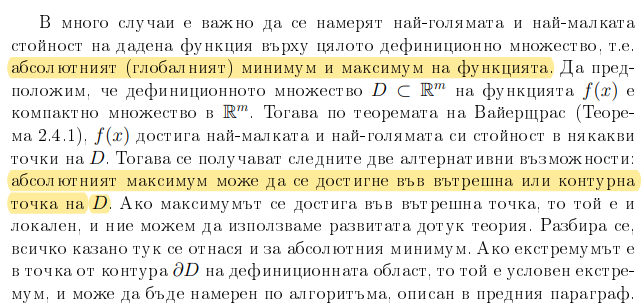
\includegraphics{Pics/calc/lec8-1.png}
  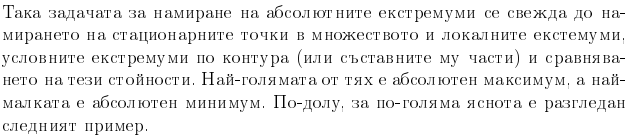
\includegraphics{Pics/calc/lec8-2.png}
\end{figure}

\begin{example}
Ако $E \subset \mathbb{R}^2, (x,y) \in \mathbb{R}^2, x \geq -1, y \geq -1, x+y \leq 1$ да се намерят най малката и най голямата стойност на функцията $f(x,y) = x^2 + y^2$ върху Е.\\
Решение:
\begin{gather*}
M_0 = (0,0) \in E \\
\Delta = 2 \cdot 2 - 0^2 >0 \quad f''_{xx} = 2 > 0 \implies f_{min} \\
f_{min} = f(0,0) = 0 \\
L(x,y;\lambda) = f(x,y) + \lambda(x+y-1) = x^2 + y^2 + \lambda(x+y-1) \\
L'_x = 2x + \lambda \quad L'_y = 2y + \lambda \\
\begin{array}{|l@{}}
2x + \lambda = 0\\
2y + \lambda = 0
x+y - 1 = 0
\end{array} \Leftrightarrow 
\begin{array}{|l@{}}
x = - \frac{\lambda}{2} \\
y= - \frac{\lambda}{2} \\
\lambda  = -1
\end{array} 
\implies M_1 \left( \frac{1}{2},\frac{1}{2} \right) 
\end{gather*}

\begin{gather*}
L''_{xx} = 2 \quad L''_{yy} = 2 \quad L''_{xy} = L''_{yx} = 0 \\
f_{min} = f(M_1)  = \frac{1}{4} + \frac{1}{4} = \frac{1}{2}\\
x = -1 \Leftrightarrow g(y) = (-1)^2 + y^2 = y^2 + 1 \\
g_{min} = g(0) = 1 = f_{min} \implies M_2(-1,0)\\
y = -1 \Leftrightarrow h(x) = x^2 + (-1)^2 = x^2 + 1 \\
h_{min} = h(0) = 1 = f_{min} \implies M_3(0,-1) \quad f(M_3) = 1\\
\begin{array}{|l@{}}
x + y = 1 \\
y = -1\\
\end{array}  \implies M_4(2,-1) 
\qquad 
\begin{array}{|l@{}}
x + y = 1  \\
x = -1\\
\end{array}  \implies M_5(-1,2) \\
f(-1,-1) = 2  \quad f(2,-1) = 5 \quad f(-1,2) = 5
\end{gather*}

\end{example}

\newpage
\section{Лекция 9: Двоен интеграл}

\subsection{Понятие за обем в $\mathbb{R}^m$. Множество с мярка нула}
Нека $T_k (k=0,1,2...)$ е съвкупността от всички затворени кубове от вида 
$$Q^m = Q^{m,k} = \left \{ x: x \in \mathbb{R}^m,  \frac{l_i}{10^k} \leq x_i \leq  \frac{l_i + 1}{10^k}, i = 1,2,...,m \right \}$$
където $l_i \in \mathbb{Z}$ За удобство кубовете се означават просто $Q^m$.

\begin{definition}
Системата $T_k$ се нарича разделяне на $\mathbb{R}^m$ от ранг k, а кубовете $Q^m$ - кубове от ранг k.
\end{definition}
В частност за $m = 1$ множествата $Q^m$ са интервали, а за $m = 2$ -  квадрати. По нататък ще предполагаме, че $m \geq 2$
\begin{definition}
Числото $\frac{1}{10^{km}}$ се нарича m-мерен обем на куба $Q^m$ и е използвано означението $\mu(Q^m)$.
$$\mu(Q^m) = \frac{1}{(10^k)^m} = \frac{1}{10^{km}}, k = 0,1,2,...$$
\end{definition}
 
\begin{definition}
Ако $E \subset \mathbb{R}^m$ и Е представлява обеднинение на крайно или изброимо много кубове $Q_j ^m$ от даден ранг k, т.е. $E = \cup_j Q_j ^m$, то $\mu(E)$ се дефинира като 
$$\mu(E) = \sum_j \mu(Q_j ^m)$$
\end{definition}
Нека $G \subset \mathbb{R}^m$ G - отворено. Да означим със $S_k = S_k(G)$ множеството от точки на всички m-мерни кубове от ранг k, изцяло лежащи в G. Тогава
$$S_0 \subset S_1 \subset S_2 \subset ... \subset S_k \subset S_{k+1} \subset ...$$
и следователно
$$\mu(S_0) \leq \mu(S_1) \leq ... \leq \mu(S_k) \leq \mu(S_{k+1}) \leq ... $$
и поради това съществува крайна или безкрайна граница $\lim\limits_{k \to \infty} \mu(S_k)$.

\begin{definition}
Крайната или безкрайната граница $\lim\limits_{k \to \infty} \mu(S_k(G))$ се нарича m-мерна мярка или m-мерен ожем на множеството G и се означава с $\mu(G)$
$$\mu(G) = \lim\limits_{k \to \infty} \mu(S_k(G))$$
\end{definition}
По силата на тази дефиниция $\mu(G) >0$ за всяко отворено непразно множество $G \subset \mathbb{R}^m$ и $\mu(G) < \infty$ ако G е и ограничено.\\

\begin{lemma}[адитивност на мярка]
Нека $G', G'' \subset \mathbb{R}^m$ са отворени множества и $G' \cap G'' = \varnothing$ тогава е в сила
$$\mu (G' \cup G'') = \mu(G') + \mu(G'')$$
\end{lemma}

\begin{lemma}[полуадитивност на мярка]
Нека $G', G'' \subset \mathbb{R}^m$ са отворени множества. Тогава е в сила
$$\mu (G' \cup G'') \leq \mu(G') + \mu(G'')$$
\end{lemma}

\begin{lemma}[адитивност на мярка]
Нека $G', G'' \subset \mathbb{R}^m$ са отворени множества и $G' \subset G''$ тогава е в сила
$$ \mu(G') \leq \mu(G'')$$
\end{lemma}

\begin{definition}
Границата $\lim\limits_{k \to \infty} \mu(S_k ^*(G))$ се нарича горна m-мерна мярка на множеството D и се означава с $\overline{\mu}(D)$
$$\overline{\mu}(D) = \lim\limits_{k \to \infty} \mu(S_k ^*(G))$$
\end{definition}

\begin{lemma}[монотонност на горната мярка]
Ако $D',D'' \subset \mathbb{R}^m$ то в сила е неравенството
$$\overline{\mu}(D') \leq \overline{\mu}(D'')$$
\end{lemma}

\begin{lemma}[полуадитивност на горната мярка]
Ако $D_i \subset \mathbb{R}^m, i = 1 \div s$ и $D = \cup_{i =1} ^s D_i$ то в сила е неравенството
$$\overline{\mu}(D) \leq \sum_{i=1}^s \overline{\mu}(D_i)$$ 
\end{lemma}

\begin{definition}
Ако $\overline{\mu}(D) = 0$ то множеството D се нарича множество с мярка нула и се записва $\mu(D) = 0$. Празното множество по дефиниция има мярка нула $\mu(\varnothing) = 0$
\end{definition}

\subsection{Измерими множества в $\mathbb{R}^m$}
Нека $G \subset \mathbb{R}^m$ е ограничено множество, $[G]$ е негова затворена обвивка. Да означим с $S_k ^* ([G])$ множеството от точки на всички m-мерни кубове от ранг k, всеки който се пресича с [G] а със $S_k (G)$ множеството от точки на всички m-мерни кубове от ранг k, съдържащи се във G. От $S_k \subset S_k ^*$ следва 
$$\mu(S_k) \leq \mu(S_k ^*)$$
откъдето при $k \to \infty$ се получава че
$$\mu(G) \leq \overline{\mu}([G])$$

\begin{definition}
Множеството $G \subset \mathbb{R}^m$ (G - отворено и ограничено) се нарича измеримо(кубируемо, а при $m = 2$ - квадратируемо), ако неговата мярка е равна на горната мярка на [G]
$$\mu(G) = \overline{\mu}([G])$$
\end{definition}

\begin{theorem}
Ограниченото и отвореното множество $G \subset \mathbb{R}^m$ e измеримо, тогава и само тогава, когато контурът му има мярка нула.
$$\mu(\partial G) = 0$$
\end{theorem}

\begin{definition}
Затворената обвивка [G] на отвореното и измеримо множество $G \subset \mathbb{R}^m$ също се нарича измеримо и по дефиниция 
$$\mu([G]) = \mu(G)$$
\end{definition}

\subsection{Дефиниция на многократен интеграл}
Нека $G \subset \mathbb{R}^m$ e отворено и измеримо множество.

\begin{definition}
Системата $\tau = \{ G_i\}_{i=1}^{i_0}$ oт измерими множества $G_i$ се нарича разделяне на множеството G, ако

\begin{enumerate}
\item $G_i \subset G, i = 1 \div i_0$
\item $G_i \cap G_j = \varnothing, i \neq j$
\item $\cup[G_i] = [G]$
\end{enumerate}

\end{definition}

\begin{definition}
Числото $$\delta_{\tau} = \max_{1 \leq i \leq i_0} d(G_i)$$
Където $d(G_i)$ е диаметър на множеството $G_i$, се нарича диаметър на разделянето $\tau$
\end{definition}

\begin{lemma}
Ако $\tau = \{ G_i\}_{i=1}^{i_0}$ е разделянето на G, то
$$\mu(G) = \sum_{i=1}^{i_0} \mu(G_i)$$
\end{lemma}

\begin{definition}
Нека $\tau = \{ G_i\}$ и $\tau' = \{ G'_j\}$ са две разделяния от отвореното и измеримо множество G. Разделянето $\tau'$ се нарича вписано в $\tau$ ако за всеки елемент $G'_j \in \tau'$ съществува елемент $G_i \in \tau$, такъв че $G'_j \subset G_i$ Записва се $\tau' \succ \tau$ или $\tau \prec \tau'$.
\end{definition}

\begin{lemma}
В сила са следните свойства

\begin{enumerate}
\item Ако $\tau \prec \tau'$ и $\tau' \prec \tau''$, то $\tau \prec \tau''$ .
\item За всеки две разделяния $\tau' = \{ G'_i\}$ и $\tau'' = \{ G''_j\}$ на отвореното и измеримо множество G съществува разделяне $\tau$, такова че $\tau' \prec \tau$ и $\tau'' \prec \tau$.
\end{enumerate}

\end{lemma}

\begin{definition}
Нека $G \subset \mathbb{R}^m$, функцията $f: [G] \to \mathbb{R}$ и $\tau = \{ G_i\}_{i=1}^{i_0}$ e разделяне на множеството G. Тогава сумата 
$$\sigma_\tau (f) = \sum_{i=1} ^{i_0} f(\xi^{(i)})\mu(G_i)$$
където 
$$\xi^{(i)} \in [G_i], i = 1,2,..., i_0$$
се нарича риманова интегрална сума на функцията f. 
\end{definition}

\begin{definition}
Крайната граница 
$$\lim\limits_{\delta_\tau \to 0} \sigma_\tau (f)$$
ако съществува се нарича многократен интеграл от функцията f върху измеримото и отворено множеството G(или [G]) а функцията се нарича интегруема в риманов смисъл върху множеството G(или [G]). Означава се по един от следните начини 
$$\int f \ dG, \int f(x) \ dG, \int ... \int f(x_1, x_2,..., x_m) \ dx_1 \ dx_2 \ ... \ dx_m$$
Множеството G([G]) се нарича област на интегриране.
\end{definition}

\begin{definition}
Числото А се нарича интеграл от функцията f върху отвореното и измеримо множество G, ако за всяка редица от разделяния $\tau_n = \left \{ G_i ^{(n)}\right \}_{i=1} ^{i_0 ^{(n)}}$ на множеството G, с $\delta_{\tau_n} \to 0$ при $n \to \infty$ и каквито и да са точките
$$\xi^{(i_n)} \in [G_i ^{(n)}], i_n = 1,2,... i_0 , n = 1,2,...$$
е изпълнено равенството 
$$\lim\limits_{n \to \infty} \sigma_{\tau_n} (f;\xi_n ^{(1)}, \xi_n ^{(2)}, ..., \xi_n ^{(i_0 ^ {(n)})}) =  A$$
\end{definition}

\subsection{Съществуване на многократния интеграл}

\begin{theorem}
Нека $G \subset \mathbb{R}^m$ отворено e измеримо множество и функцията $f: [G] \to \mathbb{R}$ е интегруема върху него. Тогава f  е ограничена върху множеството [G]. 
\end{theorem}

\subsection{Свойства на многократните интеграли}
За класа на функции, интегруеми в риманов смисъл в дадено отворено и измеримо множество G е използвано означението $\Re(G)$. \\
Нека $G \subset \mathbb{R}^m$, G - измеримо и отворено множество.\\
Oсвен това $f,g: [G] \to \mathbb{R}, f,g \in \Re(G)$, a $\lambda, \nu$ - производни реални константи.

\begin{theorem}
В сила са следните свойства на многократните интеграли
\begin{enumerate}
\item $\int \ dG = \int 1 \ dG = \mu(G)$
\item $\int (\lambda f + \nu g) \ dG = \lambda \int f \ dG + \nu \int g \ dG$ (Линейност на интеграла)\\
В частност
\begin{enumerate}
\item $\lambda = \nu = 1 \implies \int (f+g) ю dG  = \int f \ dG + \int g \ dG$ 
\item $\lambda = 1,  \nu = -1 \implies \int (f-g) \ dG  = \int f \ dG - \int g \ dG$ 
\item $\lambda = const,  \nu = 0 \implies \int \lambda f \ dG  = \lambda \int f \ dG$ 
\end{enumerate}
\item $f \geq 0$ върху G $\implies \int f \ dG \geq 0$
\end{enumerate}
\end{theorem}
Oт тези три свойства се получва следствието 
$$f \geq g \implies \int f \ dG \geq \int g \ dG$$

\begin{theorem}
Ако $G', G''$ са измеримо множество, $[G] = [G'] \cup [G'']$ и $G' \cap G'' = \varnothing$ то следва
$$\int f \ dG = \int f \ d(G' \cup G'') =\int f \ dG' + \int f \ dG'' $$
\end{theorem}

\begin{theorem}[адитивност относно множества]
Ако $G' \subset G$ е измеримо множество, то $f \in \Re(G')$
\end{theorem}
Oт тази теорема следва монотонноста на интеграла: Ако $\Gamma \subset G$ е измеримо множество и $f \geq 0$ върху  G, то 
$$\int f \ dG \geq \int f \ d\Gamma$$

\begin{theorem}
Произведението $f \cdot g \in \Re(G)$
\end{theorem}

\begin{theorem}
Функцията $\vert f \vert \in \Re(G)$ и освен това е изпълнено неравенството 
$$\left \vert \int f \ dG \right \vert \leq \int \vert f \vert \ dG$$
\end{theorem}

\newpage
\subsection{Свеждане на кратни интеграли до повторни}

\subsubsection{Двумерен случай}
Нека равнината $\mathbb{R}^2$ е фиксирана правоъгълна кординатна система с кординати x и y.

\begin{definition}
Нека $G \subset \mathbb{R}^2$. G се нарича елементарна област отностно $Оу$, ако $\partial G$ се състои от графиките на две непрекъснати функции $\varphi(x), \psi(x)$, дефинирани в интервал [a,b] и $\varphi(x) \leq \psi(x), x\in [a,b]$, и може да съдържа и отсечки от правите $x = a, x = b$. Аналогично се дефинира област, елементарна отностно $Ox$.
\begin{figure}[htp!]
  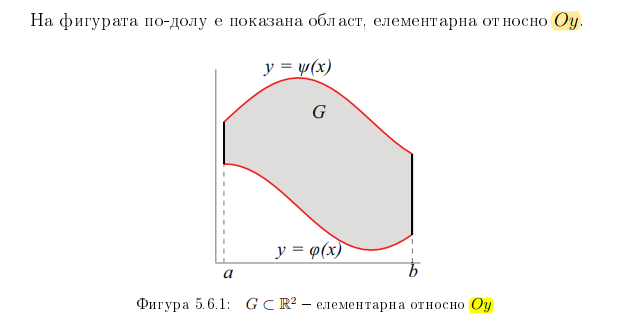
\includegraphics{Pics/calc/lec9-1.png}
\end{figure}

\end{definition}

\begin{theorem}[Теорема на Фубини]
Нека G е елементарна фигура отностно $Oy, G \subset \mathbb{R}^2, \partial G$ границата на G, се състои от графиките на непрекъснатите функции $\varphi(x) \psi(x), \varphi(x) \leq \psi(x), x\in [a,b]$ и евентуално от отсечки от правите $x = a, x = b$. Нека $f: [G] \to \mathbb{R}$ и f е непрекъсната върху [G]. Тогава
$$\iint\limits_{G} f(x,y) \ dx \ dy = \int\limits_a ^b \left( \int\limits_{\varphi(x)} ^{\psi(x)}  f(x,y) \ dy \right) \ dx$$
\end{theorem}

\begin{definition}
Интегралът в дясната страна на формулата от Теорема 9.6.1 се нарича повторен и обикновенно се записва във вида
$$\int\limits_a ^b \int\limits_{\varphi(x)} ^{\psi(x)}  f(x,y) \ dy \ dx $$ 
\end{definition}

\begin{lemma}
При предпложенията от Теорема 9.6.1 функцията 
$$F(x) = \int\limits_{\varphi(x)} ^{\psi(x)}  f(x,y) \ dy$$
е непрекъсната функция на x в интервала [a,b]. 
\end{lemma}
Aко областта G е елементарна отностно $Ox$ и границата ѝ се състои от графиките на непрекъснатите функции $\alpha (y), \beta(y), \alpha (y) \leq \beta(y), c \leq y \leq d$ и евентуално отсечки от правите $y = c, y = d$ и функцията $f(x,y)$ е непрекъсната в компактното множество [G] то е в сила формулата 
$$\iint\limits_{G} f(x,y) \, dx \, dy = \int\limits_c ^d \int\limits_{\alpha(y)} ^{\beta(y)}  f(x,y) \, dx  \,dy  $$

\begin{example}
$z = x^2y$ заградена между $y = x^2, y = 1$. \\
Имаме: $\iint\limits_{G} x^2y \,dx \, dy$, 
$G =
\begin{cases}
y = x^2 \\
y = 1
\end{cases}$ 
$$
\begin{array}{|l@{}}
y = x^2 \\
y = 1
\end{array} \implies
x^2 = 1 \implies x_{1,2} = \pm 1 
$$
Абсцисите на пресечните точки на кривата $y = x^2$ и $y = 1$. \\
Фигурата G се намира между правите $x = -1$ и $x = 1$ и освен това е оградена и от параболата $y = x^2$ и правата $y = 1$.  По точно
$$G = 
\begin{cases}
-1 \leq x \leq 1 \\
x^2 \leq y \leq 1
\end{cases}$$
Тогава 
\begin{gather*}
\iint\limits_{G} x^2y \,dx \, dy = \int\limits_{-1} ^ 1 x^2 \int\limits_{x^2} ^ 1 y \, dy \, dx  \qquad 
\left( \int\limits _{x^2} ^ 1 y \, dy  = \frac{y^2}{2}  \Big|_{x^2} ^ 1\right) \\
 \frac{1}{2} \int\limits_{-1} ^1 x^2 (1-x^4) \, dx = \frac{1}{2} \cdot 2 \int\limits_0 ^1 (x^2 - x^6) \, dx =  \\
\frac{x^3}{3} - \frac{x^7}{7} \Big|_0 ^ 1 = \frac{1}{3} - \frac{1}{7} = \frac{4}{21}
\end{gather*}

\end{example}

\newpage
\section{Лекция 10: Смяна на променливите на двоен интеграл}

\subsection{Матрица на Якоби}
Нека $x \in D \subset \mathbb{R}^m, f: D \to \mathbb{R}^n \implies y \in \mathbb{R}^m$ се задава със системата от функции
$$\begin{array}{|l@{}}
y_1 = f_1(x_1, x_2, ..., x_m) \\
y_2 = f_2(x_1, x_2, ..., x_m) \\
...\\
y_n = f_n(x_1, x_2, ..., x_m) 
\end{array}$$

\begin{definition}
Нека в точката $x^0 \in D$ съществуват първите частни производни на функциите $f_i (i = 1 \div m)$ от системата дефинирана по горе, тогава матрицата от всички частни производни в точката $x^0$
$$
\begin{bmatrix}
\frac{\partial y_1}{\partial x_1} &  \frac{\partial y_1}{\partial x_2}  & ... &\frac{\partial y_1}{\partial x_m}\\ 
\frac{\partial y_2}{\partial x_1} &  \frac{\partial y_2}{\partial x_2}  & ... &\frac{\partial y_2}{\partial x_m}\\ 
...& ... & ... & ... \\
\frac{\partial y_n}{\partial x_1} &  \frac{\partial y_n}{\partial x_2}  & ... &\frac{\partial y_n}{\partial x_m}
\end{bmatrix}
$$
се нарича матрица на Якоби за изображението $f(x)$.\\
Ако $m = n$ може да се пресметне детерминантата $J(x_1, x_2, ..., x_m)$ за матрицата на Якоби. 
$$J(f;x_1, x_2, ..., x_m) = \frac{D(y_1, y_2, ..., y_m)}{D(x_1, x_2, ..., x_m)} = 
\begin{bmatrix}
\frac{\partial y_1}{\partial x_1} &  \frac{\partial y_1}{\partial x_2}  & ... &\frac{\partial y_1}{\partial x_m}\\ 
\frac{\partial y_2}{\partial x_1} &  \frac{\partial y_2}{\partial x_2}  & ... &\frac{\partial y_2}{\partial x_m}\\ 
...& ... & ... & ... \\
\frac{\partial y_m}{\partial x_1} &  \frac{\partial y_m}{\partial x_2}  & ... &\frac{\partial y_m}{\partial x_m}
\end{bmatrix}$$
\end{definition}

\begin{definition}
Детерминанта на матрицата на Якоби се нарича още якобиан на изображението $f(x)$. Означава се  $J(x_1, x_2, ..., x_m)$ или $J(f)$
\end{definition}

\begin{definition}
Изображението $f: G \to \mathbb{R}^m (G \subset \mathbb{R}^m) $ дадено със системата 
$$\begin{array}{|l@{}}
y_1 = f_1(x_1, x_2, ..., x_m) \\
y_2 = f_2(x_1, x_2, ..., x_m) \\
...\\
y_n = f_n(x_1, x_2, ..., x_m) 
\end{array}$$
се нарича непрекъснато диференцируемо изображение, ако всички първи частни производни на $f_i (i = 1 \div m)$ съществуват в G и са непрекъснати там. 
\end{definition}

\begin{theorem}
Нека 
$$y = f(x) = \{y_i = f_i(x_1, x_2, ..., x_m), i = 1 \div m \}$$
е взаимно еднозначно непрекъснато диференцируемо изображение от отвореното множество $G \subset \mathbb{R}^m$ върху отвореното множество $ \widetilde{G} \subset \mathbb{R}^m$. Нека освен това и обратното изображение
$$x = f^{-1}(y) = \{x_i = f_i  ^{-1} (y_1, y_2, ..., y_m), i = 1 \div m\}$$
което е еднозначно непрекъснато диференцируемо изображение от своето дефиниционно множество $ \widetilde{G}$.  Тогава е в сила формулата 
$$\frac{D(y_1, y_2, ..., y_m)}{D(x_1, x_2, ..., x_m)} \cdot  \frac{D(x_1, x_2, ..., x_m)}{D(y_1, y_2, ..., y_m)} = 1$$
което може да се запише във вида
$$\frac{D(x_1, x_2, ..., x_m)}{D(y_1, y_2, ..., y_m)} = \frac{1}{\frac{D(y_1, y_2, ..., y_m)}{D(x_1, x_2, ..., x_m)}} $$
т.е якобианът на изображението, което е обратно на даденото изображение е равен  на реципрочната стойност на якобиана на даденото изображение.\\
Нито един от двата якобиана не е нула, защото произведението им е равно на 1. \\
При $m = 1$ формулата се свежда до формулата за производна на обратна функция
$$\frac{dy}{dx} = \frac{1}{\frac{dx}{dy}}$$

\end{theorem}

\begin{theorem}
Нека $G \subset \mathbb{R}^m$ e отворено множество, $f: G \to \mathbb{R}^m$
$$y = f(x) = 
\begin{array}{|l@{}}
y_1 = f_1(x_1, x_2, ..., x_m) \\
y_2 = f_2(x_1, x_2, ..., x_m) \\
...\\
y_n = f_n(x_1, x_2, ..., x_m) 
\end{array}$$
е непрекъснато диференцируемо изображение и нека точката $x^{(0)}  \in G $ а $ y^{(0)} = f(x^{(0)}) \in \mathbb{R}^m$.
Освен това, ако якобианът на това изображение е различен от нула в точката $x^{(0)}$, то съществува такива околностти $U_{x^{(0)}}, \, U_{y^{(0)}}$ съответно в точките $x^{(0)}, \, y^{(0)}$,
 че изображението f е взаимно еднозначно изображение от $U_{x^{(0)}}$ върху $U_{y^{(0)}}$, 
т.е $f: U_{x^{(0)}}, \to U_{y^{(0)}}$ и обратното му изображение е непрекъснато диференцируемо в множеството $ U_{y^{(0)}}$.
\\
\\
Следствие: Нека $G \subset \mathbb{R}^m$ е отворено множество и $F: G \to \mathbb{R}^m$ е непрекъснато диференцируема в G, а якобианът J(F) е различен от нула върху G. Тогава F(G) също е отворено множество. 
\end{theorem}

\begin{theorem}[Принцип за запазване на областта]
Образътна m-мерна област в m-мерното пространство при непрекъснато диференцируемо изображение с ненулев якобиан е област, т.е ако
\begin{enumerate}
\item $G \subset \mathbb{R}^m$ е област
\item $F: G \to \mathbb{R}^m$ e непрекъснато диференцируемо изображение
\item $J(F) \neq 0$ върху G
\end{enumerate}
то F(G) също е област. 
\end{theorem}
По нататък е разгледан въпросът за геометричен смисъл на модула на якобиана. За по голяма яснота е разгледано в $\mathbb{R}^2$. \\
Нека $G, G^* \subset \mathbb{R}^2$ са отворени множества и изображението $F: G \to G^*$, като F e зададена с двойката функции
$$x = x(u,v), \qquad y = y(u,v)$$
и предполагаме, че F удовлетворява следните условия
\begin{enumerate}
\item F е взаимно еднозначно изображение от G върху $G^*$
\item F e непрекъснато диференцируемо върху G
\item Якобианът $J(u,v) = \frac{\partial (x,y)}{\partial (u,v)} \neq 0$ върху G
\end{enumerate}
Изображението $F^{-1}$ което е обратно на F също е непрекъснато диференцируемо взаимно еднозначно изображение и якобианът му е различен от нула в $G^*$

\begin{lemma}
Ако $\gamma \subset G$ е по части гладка крива, то и нейния образ $\gamma^* = F(\gamma)$ е също по части гладка крива.
\\
\\
Забележка: Ако $\gamma \subset G$ е прост затворен контур, то поради взаимната еднозначност на F, неговия образ $\gamma^* = F(\gamma)$ е също прост затворен контур. 
\end{lemma}


\begin{lemma}
Ако $\Gamma$ е отворено и ограничено множество и $[\Gamma] \subset G$ тогава $\Gamma^* = F(\Gamma)$ е също отворено и ограничено множество и 
$$\partial F(\Gamma) = F(\partial \Gamma)$$
Aко $\partial \Gamma$ се състои от краен брой по част гладки криви, то отворените множества $\Gamma$ и $F(\Gamma)$ са квадрируеми. 
\end{lemma}
Нека $(u_0, v_0) \in G$ и $h \in \mathbb{R}$ е реално число, и да разгледаме затворения квадрат S с върхове 
$$A(u_0, v_0) \qquad B(u_0+h, v_0) \qquad C(u_0 + h, v_0 + h) \qquad D(u_0, v_0 + h)$$
Нека $S \subset G$ (за "достатъчно малки" h това включване винаги се изпълнява). 
Границата $\partial S$ на квадрата S която се състои от четирите му страни е прост затворен по части гладък контур. 
Поради Лема 10.1.2 множеството $S^* = F(S)$ е затворена квадратируема област (факта, че $S^*$ е затворена област, следва от принципа за запзаване на областа). В сила е следната теорема

\begin{theorem}
Нека изображението F от отвореното множество $G \subset \mathbb{R}^2$ върху отвореното множество $G^* \subset \mathbb{R}^2$ е взаимно еднозначно и непрекъснато диференцируемо върху G и нека якобианът му $J(u,v) \neq 0 $ върху G.
Тогава ако S е квадрат с върховете по горе, то
$$\frac{\mu(F(S))}{\mu(S)} = \vert J(u_0,v_0)\vert + \varepsilon (u_0, v_0, h)$$
където $\varepsilon = \varepsilon (u_0, v_0, h)$ клони към нула, когато $h \to 0$. При това сходимостта е равномерна отностно $(u_0, v_0)$, върху всяко затворено и ограничено множество $A \subset G$ за което $(u_0, v_0) \in A$.\\
\\
Следствие: За всяка точка $(u_0, v_0)$ на отворено множество G е изпълнено равенството 
$$\lim\limits_{h \to 0} \frac{\mu(F(S))}{\mu(S)} = \vert J(u_0,v_0)\vert  $$
\end{theorem}
В общия случай за m-мерно пространство тази теорема се обобщава по следния начин.

\begin{theorem}
Нека множествата $G, G^* \subset \mathbb{R}^m$ са отворени множества и изображението $F: G \to G^*$, е зададено с m-торка функции
$$x = F(t) = \{x_i = x_i(t_1,t_2, ..., t_m), i = 1 \div m \}$$
Нека F е взаимно еднозначно и непрекъснато диференцируемо върху G и якобианът му
$$J(t) = \frac{\partial (x_1, ..., x_m)}{\partial (t_1, ..., t_m)} \neq 0, \quad t \in G$$
а S е m-мерния куб
$$S - \{t: t_i ^0 \leq t_i \leq t_i ^ 0 + h, i = 1, 2, ..., m \} \subset G, t^0 = (t_1 ^0, t_2 ^0, ..., t_m ^0)$$
Тогава 
$$\lim\limits_{h \to 0} \frac{\mu(F(S))}{\mu(S)} = \vert J(t^0)\vert  $$
при това, ако 
$$\frac{\mu(F(S))}{\mu(S)} = \vert J(t^0)\vert + \varepsilon (t^0, h)$$
то за всяко ограничено и затворено множество $A \subset G$, функцията $\varepsilon = \varepsilon (t^0,h)$, дефинирана за $t^0 \in A$, клони равномерно към нула върху множеството A, при $h \to 0$.
\\
\\
Ако $G,G^* \subset{R}^3, \quad F:G \to G^*$ е зададено с тройка функции
$$x= x(u,v,w) \qquad y= y(u,v,w) \qquad  z= z(u,v,w) $$
\end{theorem}

\begin{lemma}
Ако $S \subset G$ е по части гладка повърхнина в $\mathbb{R}^3$, то и нейния образ $S^* = F(S)$ е също по части гладка повърхнина. 
\\
\\
Забележка: Ако $S \subset G$ е проста затворена повърхнина, то поради взаимната еднозначност на F, неговия образ $S^* = F(S)$ е същопроста затворена повърхнина. 
\end{lemma}

\begin{lemma}
Ако $\Gamma$ е отворено и ограничено множество и $[\Gamma] \subset G$ тогава $\Gamma^* = F(\Gamma)$ е също отворено и ограничено множество и 
$$\partial F(\Gamma) = F(\partial \Gamma)$$
Aко $\partial \Gamma$ се състои от краен брой по част гладки повърхнини, то отворените множества $\Gamma$ и $F(\Gamma)$ са измерими. 
\end{lemma}

\newpage
\subsection{Смяна на променливите в многократен интеграл}
Нека
\begin{itemize}
\item F е непрекъснато диференцируемо изображение от отвореното множество $G \subset \mathbb{R}^2$ върху отвореното множество $G^2 \subset \mathbb{R}^2$
\item Якобиан $J(F) \neq 0$ в G
\item $\Gamma, \Gamma^*$ са квадратируеми (следователно ограничени) и отворени множества 
\item $[\Gamma] \subset G, [\Gamma^*] \subset G^*$
\item $F([\Gamma]) = [\Gamma^*]$
\item F изобразява вътрепните точки на $\Gamma$ във вътрешни точки на $\Gamma^*$ а контура $\partial \Gamma$ - в контура $\partial \Gamma^*$
\end{itemize}

\begin{theorem}[за смяна на променливите на двукратен интеграл]
Нека функцията 
$$f: [\Gamma^*] \to \mathbb{R}$$
е непрекъсната върху $[\Gamma]$. Тогава в сила е формулата
$$\iint\limits_{\Gamma^*} f(x,y) \, dx \, dy = \iint\limits_{\Gamma} f(x(u,v),y(u,v)) \left| \frac{\partial (x,y)}{\partial (u,v)} \right| \, du \, dv$$
\end{theorem}
Верността на (10.2.1) остава в сила и при малко по-общия случай, когато якобианът на изображението F, става нула върху границата на областта на интегриране, а самото изображение не е взаимно еднозначно върху тази граница. По-точно е в сила следната теорема.
\begin{theorem}
Нека $G,G^* \subset \mathbb{R}^2$ са отворени измерими множества и 
$$x = x(u,v), \qquad y = y(u,v)$$
е непрекъснато изображение от [G] върху $[G^*]$, което е взаимно еднозначно и непрекъснато диференцируемо изображение от G върху $G^*$. Нека якобианът на това изображение
$$J(u,v) = \frac{\partial (x,y)}{\partial (u,v)}$$
е различен от нула в G и е непрекъснато продължим върху [G]. Нека освен това функцията 
$$f: [G^*] \to \mathbb{R}$$
е непрекъсната върхи множеството $[G^*]$. Тогава е в сила формулата
$$\iint\limits_{G^*} f(x,y) \, dx \, dy = \iint\limits_{G} f(x(u,v),y(u,v) \left| \frac{\partial (x,y)}{\partial (u,v)} \right| \, du \, dv$$
\end{theorem}

\begin{example}
Да се пресметне интеграла
$$\iint\limits_{x^2+y^2 < 1} \cos (\pi \sqrt{x^2 + y^2}) \, dx \, dy$$
Нека въведем нови променливи $\rho, \varphi$ по формулите
$$x = \rho \cos \varphi \qquad y = \rho \sin \varphi $$
Тогава модулът на якобиана на смяната се дава със израза 
$$\Delta = |J(\rho, \varphi)| = \rho$$
Изображението на новите променливи е правоъгълника
$$G = \{ (\rho, \varphi): 0 < \rho < 1, -\pi < \varphi < \pi \}$$
взаимно еднозначно и непрекъснато диференцируемо и с якобиан, различен от нула върху кръга
$$K: \{ (x,y):x^2 + y^2 < 1 \}$$
от който е премахнат радиусът, лежащ върху отрицателната част на оста $Ox$, т.е G се изобразява върху множеството
$$G = K \setminus \{ (x,y) : x \leq 0, y=0\}$$
Освен това изображението на смяната изобразява затвореният правоъгълник $[G]$ върху затворения кръг
$$[G] = [K] = \{ (x,y): x^2 + y^2 < 1 \}$$
при което контура $[G]$ вече не е взаимно еднозначно. Якобианът на изображението на смяната е непрекъснат върху $[G]$ а в една точка от контура(кординатното начало) е нула. Следователно това изображение удовлетворява всички условия от Теорема (10.2.2), и затова може да се приложи формулата за смяна на променливите на интеграла. Така се получава
\begin{gather*}
\iint\limits_{x^2+y^2 < 1} \cos (\pi \sqrt{x^2 + y^2}) \, dx \, dy = \iint\limits_{G} \rho \cos(\pi \rho) \, d\rho \, d \varphi = \int\limits_{-\pi} ^{\pi}  \int\limits_0 ^1 \rho \cos(\pi \rho) \, d\rho \, d\varphi= - \frac{4}{\pi}
\end{gather*}
\end{example}


\begin{theorem}
Нека $G,G^* \subset \mathbb{R}^m$ са отворени кубируеми множества. Нека $F: [G] \to [G^*] $ е непрекъснато изображение, зададено с уравненията 
$$x = F(t) = \{x_i = x_i(t_1,t_2, ..., t_m), i = 1 \div m \}$$
взаимно еднозначно и непрекъснато диференцируемо върху G, и якобианът му
$$J(t) = \frac{\partial (x_1, ..., x_m)}{\partial (t_1, ..., t_m)} \neq 0, \quad t \in G$$
е непрекъснато продължим върху [G]. Тогава, ако функцията 
$$f: [G^*] \to \mathbb{R}$$
е непрекъсната върху $[G^*]$ то
$$\int f(x) \, dG^* = \int f(x(t)) \vert J(t) \vert dG$$
\end{theorem}

\subsubsection{Полярна смяна}
При $m = 2$ често използвана е полярна смяна, зададена с равенства 
$$F(\rho, \varphi) = \begin{cases} x = \rho \cos \varphi \\  y = \rho \sin \varphi \end{cases}$$
За да се опише $\mathbb{R}^2$, променливите $\rho, \varphi$ се изменят както следва 
$$\rho \geq 0 \qquad 0 \leq \varphi < 2\pi$$
я якобианът има стойност
$$J(\rho, \varphi) = \begin{vmatrix} x'_{\rho} &   x'_{\varphi} \\  y'_{\rho} &  y'_{\varphi}\end{vmatrix} = \rho \cos^2 \varphi + \rho \sin^2 \varphi = \rho$$
А неговия модул 
$$\Delta = |J(\rho, \varphi)| = \rho $$
Една обощена полярна смяна е следната 
$$F(\rho, \varphi) = \begin{cases} x = a\rho \cos \varphi \\  y = b\rho \sin \varphi \end{cases} \qquad (a,b > 0)$$
известна като обобщена полярна смяна, за която в общия случай
$$\rho \geq 0 \qquad 0 \leq \varphi < 2\pi$$
А неговия модул 
$$\Delta = |J(\rho, \varphi)| = ab\rho $$
Друга обощена полярна смяна е следната 
$$F(\rho, \varphi) = \begin{cases} x = a\rho \cos^k \varphi \\  y = b\rho \sin^k \varphi \end{cases} \qquad (a,b > 0m k = 2, 3, ...)$$
известна също като обобщена полярна смяна, за която в общия случай
$$\rho \geq 0 \qquad 0 \leq \varphi < 2\pi$$
А неговия модул 
$$\Delta = |J(\rho, \varphi)| = abk\rho |\cos^{k-1} \varphi \sin^{k-1} \varphi|$$
\begin{example}
Да се пресметне лицето на фигурата
$$A^* = \{(x,y) : x^{\frac{2}{3}} + y^{\frac{2}{3}} \leq a^{\frac{2}{3}}, a>0\}$$
\begin{center}
  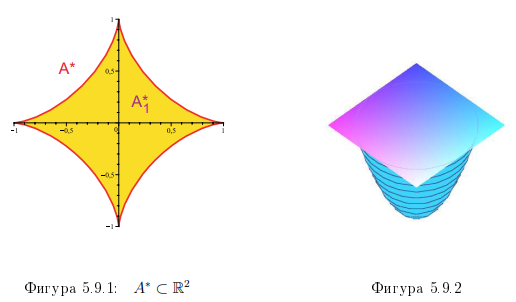
\includegraphics{Pics/calc/lec10-1.png}
\end{center}
Поради симетрията на дадената фигура, нейното лице може да се пресметни като първо се намери лицето на часта $A_1 ^*$ разположена в първи квадрант и получения резултат да се умножи по 4. За да се пресметне това може да се извърши следната смяна
$$x = \rho \cos^3 \varphi \qquad y = \rho \sin^3 \varphi $$
която води до ограничения $0 \leq \rho \leq a, 0 \leq \varphi \leq 2\pi, \quad (\rho, \varphi ) \in A$ и има якобиан с модул
$$\Delta = |J (\rho, \varphi ) | = 3\rho \cos^2 \varphi \sin^2 \varphi $$
поради което 
\begin{gather*}
\mu(A^*) = 4\mu(A_1 ^*) = 4 \iint\limits_{A_1 ^*} = 12 \int\limits_{0} ^{\frac{\pi}{2}} \cos^2 \varphi \sin^2 \varphi \, d\varphi \int\limits_0 ^a \rho \, d\rho = \frac{3\pi a^2}{8}
\end{gather*}
\end{example}

\newpage
\section{Лекция 11: Пресмятане на тройни интеграли}

\subsection{Пресмятане на тройни интеграли, чрез свеждане до повторни интеграли}
Нека $\mathbb{R}^3 = \{(x,y,z), x \in \mathbb{R}, \, y \in \mathbb{R}, \, z \in \mathbb{R}\}$. Нека областта $G \subset \mathbb{R}$ и D е нейна ортогонална проекция върху равнината $xOy$. т.е $D \subset \mathbb{R}^2$ или
$$D = \{ (x,y): \exists z, (x,y,z) \in G \}$$

\begin{definition}
Областта $G$ се нарича елементарна отностно оста $Oz$ ако нейната проекция $D$ е кубируема (измерима), а границата ѝ се състои от две функции $\varphi(x,y) \, \psi(x,y)$, непрекъснати върху множеството такива че 
$$\varphi(x,y) \leq \psi(x,y) \qquad (x,y) \in D$$
и евентуално част от цилиндъра с онсова границата $\partial D$ на проекцията $D$. \\
\end{definition}

\begin{itemize}
\item Ако $G$ е елементарна отностно oста $Oz$, то тя е измерима. \\
Нейната проекция $D$ е измерима област, следователно ограничена. 
Поради това границата на областта $G$, койято се състои от графиките на непрекъснатите функции върху компактното множество $[D]$ и евентуално част от цилиндър с основа, която има мярка нула
$$\mu(\partial D) = 0$$
\item Ако 
$$f: [G] \to \mathbb{R}$$
е непрекъсната функция, то Теоремата на фубини се обобщава и е валидна следната формула
$$\iiint\limits_G f(x,y,z) \, dx \, dy \, dz = \iint\limits_G \, dx \, dy \int\limits_{\varphi(x,y)} ^{\psi(x,y)} f(x,y,z) \, dz =  \iint\limits_G \left[ \int\limits_{\varphi(x,y)} ^{\psi(x,y)} f(x,y,z) \, dz  \right]\, dx \, dy $$
\end{itemize}

\newpage
\begin{example}
Нека $\iiint\limits_T \, dx \, dy \, dz$ по ограничената област Т, заградена от повърхнините с уравнения $x=0, \, y=0, \, z=0, \, x+y+z=1$.
\begin{center}
  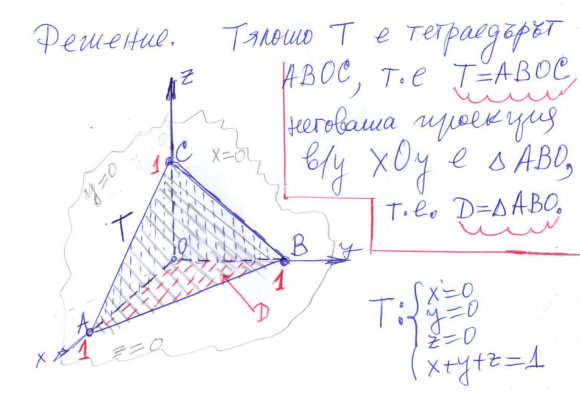
\includegraphics[width = \linewidth]{Pics/calc/lec11-1-1.png}
\end{center}
Повърхнината $x+y+z = 1$ е равнина пресичаща и трите кординатни оси с отрези от тях равни на 1. $x=0, \, y=0, \, z=0$ са кординатните равнини. Проекцията на D на тялото се получава от 
$$\begin{cases} x+y+z = 1 \\ x=0 \\y=0 \\ z= 0 \end{cases} \implies D: \begin{cases} x+y= 1 \\ x=0 \\y=0 \end{cases}$$
\begin{center}
  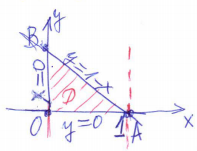
\includegraphics{Pics/calc/lec11-1-2.png}
\end{center}
Имаме
$$A: \begin{array}{|l@{}} y = 1 - x \\ y=0 \end{array} \implies A(1,0) \implies \begin{cases} 0 \leq x \leq 1 \\ 0 \leq y \leq 1-x \end{cases}$$
По нататък 
$$0 \leq z \qquad x+y+z \leq 1 \implies 0 \leq z \leq 1 - x - y$$
Тогава получаваме 
\begin{gather*}
\iiint\limits_T \, dx \, dy \, dz = \int\limits_0 ^1 \int\limits_0 ^{1-x} \int\limits_0 ^{1-x-y} \, dz \, dy \, dx  \\
\int\limits_0 ^{1-x-y} \, dz = z\Big|_0 ^{1-x-y} = 1-x-y \\
I =  \int\limits_0 ^1 \int\limits_0 ^{1-x} 1-x-y \, dy \, dx \\
\int\limits_0 ^{1-x} 1-x-y \, dy = (1-x) \Big|_0 ^{1-x} - \frac{y^2}{2}  \Big|_0 ^{1-x} = \frac{(1-x)^2}{2} \\
I = \frac{1}{2} \int\limits_0 ^1 (1-x)^2 \, dx =  \frac{1}{2} \int\limits_0 ^1 (x-1)^2 \, dx =   \frac{1}{2} \int\limits_0 ^1 (x-1)^2 \, d(x-1) \\
I = \frac{1}{2} \frac{(x-1)^3}{3} \Big|_0 ^1 = \frac{1}{6} [0 - (-1)^3] = \frac{1}{6}
\end{gather*}
\end{example}

\subsection{Приложение на многократните интеграли}
Нека $G \subset \mathbb{R}^m$ е измеримо (кубируемо) множество. Както е известно от Теорема (9.5.1) мярката на G се изразява с формулата по долу
$$\mu (G) = \int \, dG$$
По такъв начин посредством m-кратен интеграл може да се пресметне мярката на кубируемо множество в m-мерното простраство(лице - в двумерно, обем - в тримерното пространства). Ако m-кратнията интеграл може да се сведе до повторен, то пресмятането на мярката на кубируемото множество G, се свежда до пресмятане на (m-1)-кратен интеграл. \\
Ако $m=2$, площта на измеримата на равнинна област $D \subset \mathbb{R}^2$ се пресмята по формулата 
$$S(D) = \mu(D) = \iint\limits_D \, dx \, dy$$
Ако $m=3$, обема на измеримата на равнинна област $T \subset \mathbb{R}^3$ се пресмята по формулата 
$$V(T) = \mu(T) = \iiint\limits_T \, dx \, dy \, dz$$
Освен това този интеграл може да се сведе до повторен и D е проекция на тялото T върху $\mathbb{R}^2$ а, Т e разположено повърхнините $z = f_1(x,y) \, z = f_2 (x,y)$ като е изпълнено неравенството $ f_1(x,y) \leq f_2 (x,y), \quad (x,y) \in D$ формулата за обем може да се запише
$$V(T) = \mu(T) = \iint\limits_D \left[ f_2 (x,y) - f_1 (x,y)\right] \, dx \, dy$$
Друга полезна формула е тази за намиране на част от повърхнина заключена в цилиндрична повърхнина. С други думи, ако $D \subset \mathbb{R}^2$ е квадратируема област и повърхнината S е дефинирана в затвореното множество $[D]$
$$S: z = f(x,y) \qquad f:[D] \to \mathbb{R}$$
Като при това f е непрекъснато диференцируема в D, то лицето на тази повърхнина се дава с формулата
$$\sigma = \sigma(S) = \iint\limits_D \sqrt{1 + (z'_x)^2 + (z'_y)^2} \, dx \, dy$$

\begin{example}
Да се пресметне лицето на частта от повърхнината $S: z = \sqrt{x^2 + y^2}$, разположена във вътрешността на цилиндрична повърхнина с уравнение $x^2 + y^2 = 2x$ \\
D е отворения кръг с център точката (1,0) и радиус 1, защото 
$$x^2 + y^2 = 2x \Leftrightarrow (x-1)^2 + y^2 = 1$$
Oсвен това
$$z'_x = \frac{x}{\sqrt{x^2 + y^2}} \qquad z'_y = \frac{y}{\sqrt{x^2 + y^2}} \qquad \sqrt{1 + (z'_x)^2 + (z'_y)^2} = \sqrt{2}$$
Oт формулата имаме
$$\sigma = \sigma(S) = \iint\limits_D \sqrt{2}\, dx \, dy =  \sqrt{2} \iint\limits_D \, dx \, dy = \sqrt{2} \mu(D) = \sqrt{2} \pi $$
\end{example}

\subsection{Смяна на променливите на троен интеграл}

\begin{theorem}
Нека $G,G^* \subset \mathbb{R}^3$ са отворени измерими множества. Нека $F: [G] \to [G^*]$ е непрекъснато изображение зададено чрез системата функция
$$F(u,v,w) = \begin{cases} x = x(u,v,w) \\ y = y(u,v,w) \\ z = z(u,v,w)\end{cases}$$
взаимно еднозначно и непрекъснато диференцируемо изображение от G върху $G^*$. Нека якобианът на това изображение
$$J(u,v,w) = \frac{D(x,y,z)}{D (u,v,w)} = \begin{vmatrix} x'_u & x'_v & x'_w \\  y'_u & y'_v & y'_w \\ z'_u & z'_v & z'_w \end{vmatrix} \neq 0 \quad (u,v,w) \in G$$
е непрекъснато продължим върху [G]. Нека освен това функцията 
$$f: [G^*] \to \mathbb{R}$$
е непрекъсната върхи множеството $[G^*]$. Тогава е в сила формулата
$$\iiint\limits_{G^*} f(x,y) \, dx \, dy = \iiint\limits_{G} f(x(u,v,w),\,y(u,v,w),\,z(u,v,w)) |J(u,v,w) | \, du \, dv \, dw$$
\end{theorem}

\subsubsection{Цилиндрична смяна}
Честно използвани смени на променливите при тройни интеграли са цилиндричната смяна, зададена с уравнения
$$F(\rho, \varphi, z) = \begin{cases} x = \rho \cos \varphi \\  y = \rho \sin \varphi  \\ z = z \end{cases}$$
и обобщена цилиндрична смяна 
$$F(\rho, \varphi, z) = \begin{cases} x = a\rho \cos \varphi \\  y = b\rho \sin \varphi  \\ z = z \end{cases} \quad (a,b > 0)$$
За да се опише цялото $\mathbb{R}^3$, диапазонът на изменение на променливите е както следва 
$$\rho \geq 0 \qquad 0 \leq \varphi < 2\pi \qquad -\infty < z < \infty$$
А неговия модул съответно
$$\Delta = |J(\rho, \varphi, z)| = \rho \qquad \Delta = |J(\rho, \varphi, z)| = ab\rho $$

\subsubsection{Сферична смяна}
Друга смяна е сферичната смяна, зададена с уравнения 
$$F(\rho, \varphi, \psi) = \begin{cases} x = \rho \sin \psi \cos \varphi \\  y = \rho \sin \psi \sin \varphi  \\ z = \rho \cos \psi \end{cases}$$
За да се опише цялото $\mathbb{R}^3$, диапазонът на изменение на променливите е както следва 
$$0 \leq \rho \qquad 0 \leq \varphi < 2 \pi \qquad 0 \leq \psi \leq \pi$$
a модула на якобиана се дава с равенсвото
$$\Delta = |J(\rho, \varphi, \psi)| = \rho^2 \sin \psi$$
Понякога се дава и следната вариация на сферична смяна
$$F(\rho, \varphi, \theta) = \begin{cases} x = \rho \cos \theta \cos \varphi \\  y = \rho \cos \theta \sin \varphi  \\ z = \rho \sin \theta \end{cases}$$
с диапазон на изменение на променливите
$$0 \leq \rho \qquad 0 \leq \varphi < 2 \pi \qquad -\frac{\pi}{2} \leq \psi \leq \frac{\pi}{2}$$
и модул на якобиана
$$\Delta = |J(\rho, \varphi, \theta)| = \rho^2 \cos \theta$$

\begin{example}
Да се пресметне обемът на тялото
$$T^* = \{ (x,y,z) : x^2 + y^2 \leq z, \, z \leq 4\}$$
Ако направим цилиндрична смяна получаваме
$$\mu(T^*) = \iiint\limits_{T^*} \, dx \, dy \, dz = \int\limits_ 0 ^{2\pi} \int\limits_ 0 ^{2} \rho \int\limits_ {\rho^2} ^{4} \, dz \, d\rho \, d\varphi = 8\pi$$
Проекцията $D^* \text{ на } T^*$ върху $xOy$ се определя от 
$$x^2 + y^2 \leq z, \quad z \leq 4 \implies x^2 + y^2 \leq 4 \implies D^* \{ (x,y) : x^2 + y^2 \leq 4 \}$$
От $D^*$ се определят границите за x и y. \\
Границите за променливата z са
$$x^2 + y^2 \leq z \leq 4$$
След цилиндричната замяна се получава
$$x^2 + y^2 = \rho^2 \cos^2 \varphi + \rho^2 \sin^2 \varphi  = \rho^2 ( \cos^2 \varphi +  \sin^2 \varphi) = \rho^2 \leq 4 $$
$$\rho^2 \leq 4 \qquad \rho > 0 \implies 0 \leq \rho \leq 2 $$ 
$$x^2 + y^2 \leq z \leq 4 \implies \rho^2 \leq z \leq 4 $$
а $\varphi$ остава в $0 \leq \varphi < 2 \pi$, защото няма нови ограничения. 
\end{example}

\newpage
\section{Лекция 12: Kриви и повърхнини в тримерното пространство}

\subsection{Kриви и повърхнини в тримерното пространство}
Нека $\Gamma \subset \mathbb{R}^3$ e непрекъсната крива линия, зададена в следния параметричен вид: 
$$\Gamma: \{r(t); t \in [\alpha, \beta] \} \equiv \{x = \varphi(t), y = \psi(t), z = \chi(t) ; t \in [\alpha, \beta] \}$$
в интервала $[\alpha, \beta] \subset \mathbb{R}$.

\begin{definition}
Точката $A = r(\alpha)$ се нарича начало на кривата, а $B = r(\beta)$ - неин край.
\end{definition}

\begin{definition}
Точка от кривата $\Gamma$, която е образ на повече от една точка от интервала $[\alpha, \beta]$ (с изключение на началото и края) се нарича точка на самопресичане или кратна точка на тази крива. 
Крива която няма други точки на самопресичане (освен $r(\alpha) = r(\beta)$) и такива, че $r(t) \neq r(\alpha) = r(\beta); t \in [\alpha, \beta] $ се нарича прост контур. 
Кривата $\Gamma$ се нарича затворена крива или затворен контур, ако началото ѝ съвпада с нейния край, $r(\alpha) = r(\beta)$.
\end{definition}

\begin{definition}
В частност ако кривата $\Gamma$ лежи в някаква равнина, тя се нарича равнинна. 
Ако посочената равнина е кординатната равнина $xOy$, то представянето на тази крива има вида 
$$\Gamma: \{r(t); t \in [\alpha, \beta] \} \equiv \{x = \varphi(t), y = \psi(t), z = 0 ; t \in [\alpha, \beta] \}$$
при което уравнението $z = 0$ обикновенно не се пише.
\end{definition}

\begin{definition}
Кривата $\Gamma$ се нарича диференцируема, ако кординатните ѝ функции $ \varphi(t), \psi(t), \chi(t)$ са диференцируеми в $[\alpha, \beta]$, а
$$r'(t) = ( \varphi'(t), \psi'(t), \chi'(t))$$
се нарича производна на представянето $r(t)$ на кривата. Ако освен това тези функци са и непрекъснато диференцируеми, то кривата се нарича непрекъснато диференцируема. 
\end{definition}

\begin{definition}
Нека кривата $\Gamma$ е диференцируема крива. 
Точката на кривата $\Gamma$ в която $r' \neq 0$ се нарича неособена, а точката в която $r'=0$ - особена.
\end{definition}
От равенството
$$|r'| = \sqrt{ \varphi'^2 + \psi'^2 + \chi'^2}$$
следва че точката $( \varphi(t), \psi(t), \chi(t))$ от кривата $\Gamma$ е неособена тогава и само тогава когато $\varphi'^2 (t)+ \psi'^2 (t) + \chi'^2 (t) > 0$ т.е поне една от производните е различна от нула. \\
Кривата $\Gamma$ има допирателна във всяка неособена точка. 

\begin{definition}
Кривата $\Gamma$ се нарича гладка, ако е непрекъснато диференцируема крива без особени точки.
Ако дадената крива не е гладка, но може да се представи като сума от краен брой гладки криви, се казва, че тя по части гладка или частично гладка. 
\end{definition}

\begin{definition}
Кривата се нарича ректифицируема, ако има крайна дължина. 
\end{definition}

\begin{definition}
Множеството $D \subset \mathbb{R}^2$ се нарича едносвързано, ако за всяка непрекъсната затворена крива линия $\gamma \subset D$ е изпълнено $Int \gamma \subset D$, където $Int \gamma$ е множеството от всички точки, които се намират в ограниченото множество $\widetilde{D}$ с контур $\partial \widetilde{D} = \gamma$
\end{definition}
Нека сега $D \subset \mathbb{R}^2$ е едносвързана област и за всички точки от тази област са дефинирани три функции
$$x = x(u,v) \qquad y = y(u,v) \qquad  z = z(u,v) $$
или векторна функция 
$$r = r(u,v)$$
където $r(u,v)$ е вектор с компоненти $x = x(u,v) \, y = y(u,v) \, z = z(u,v)$.

\begin{definition}
Казва се че уравненията по горе (x,y,z) или (r) дефинират гладка повърхност, ако функциите (x,y,z) са непрекъснато диференцируеми в областта D и векторното произведение 
$$N = r'_u (u,v) \times r'_v (u,v) \neq 0 \qquad (u,v) \in D$$
а векторите 
$$N = r'_u (u,v) \times r'_v (u,v), \qquad n = \frac{N}{\Vert N \Vert}$$
се наричат съответно нормален вектор (нормала) и единичен нормален вектор към тази повърхнина.
Ако повърхнината не е гладка, но може да се раздели на краен брой гладки части, тя се нарича частично гладка или по части гладка повърхнина.
\end{definition}

\begin{example}[Лист на Мьобиус]
Ако залепим правоъгълника $ABCD$ така, че А да съвпада с C, а B с D то че получава повърхнина, известна като лист на Мьобиус.
 Нейната нормала се характеризира с това, че след като направи една обиколка, тя сменя посоката си с противоположната. 
\end{example}

\newpage
\section{Лекция 13: Криволинейни интеграли}

\subsection{Дефиниция на криволинейни интеграли от първи и втори род}
Нека функциите $f(x,y,z), P(x,y,z), Q(x,y,z), R(x,y,z)$ са дефинирани върху непрекъснатата проста ректифируема крива $\Gamma$ с началнa точка A и крайна точка B. 
\begin{center}
  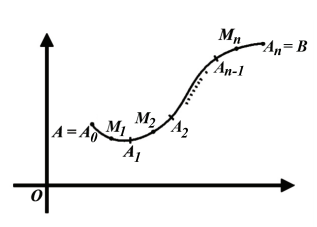
\includegraphics{Pics/calc/lec13-1.png}
\end{center}
С помощта на точките $A \equiv A_0, A_1, ..., A_n \equiv B$ с кординати съответно $A_i(x_i,y_i,z_i) (i=0,1,...,n)$, кривата $\Gamma$ е разделеня на n дъгички и върху всяка дъгичка произволно е избрана точка $M_i (\xi_i,\eta_i,\zeta_i)$, в която се пресмятат стойностите $f(\xi_i,\eta_i,\zeta_i), P(\xi_i,\eta_i,\zeta_i), Q(\xi_i,\eta_i,\zeta_i), R(\xi_i,\eta_i,\zeta_i)$ на функциите $f, P, Q, R$. 
Да отбележим, че аналогичен процес на разделяне може да бъде проведен и в случай на затворена крива, ако за точка $A_0 (A_n)$ се вземе коя да е нейна точка, а останалите точки $A_i$ да се разположат последователно по кривата в една от двете възможни посоки. \\
За дължината на i-тата дъгичка е използвано означението $\Delta l_i$, а за дължината на най-дългата дъгичка от разделянето $\delta_n$
$$\Delta l_i = \text{дължината на } A_{i-1} A_i \qquad \delta_n = \max\limits_{i = 1\div n} \Delta l_i$$
Наред с това са въведени и означенията 
$$\Delta x_i = x_i - x_{i-1} \qquad \Delta y_i = y_i - y_{i-1} \qquad \Delta z_i = z_i - z_{i-1} \qquad i = 1 \div n $$
По нататък са образувани съответните интегрални суми за всяка една от разглежданите функции както следва
\begin{gather*}
\sigma_n (f) = \sum_{i=1} ^n f(\xi_i,\eta_i,\zeta_i) \Delta l_i \\
\sigma_n (P) = \sum_{i=1} ^n P(\xi_i,\eta_i,\zeta_i) \Delta x_i  \\
\sigma_n (Q) = \sum_{i=1} ^n Q(\xi_i,\eta_i,\zeta_i) \Delta y_i  \\
\sigma_n (R) = \sum_{i=1} ^n R(\xi_i,\eta_i,\zeta_i) \Delta z_i  \\
\end{gather*}

\begin{definition}
Границата на интегралната сума (първата; ако съществува, не зависейки нито от начина на разделяне, нито от избора на точките $M_i$) при $\delta_n$, клоняща към нула се нарича криволинеен интеграл от първи род на функцията $f(x,y,z)$ върху кривата $\Gamma$ и се записва $\int\limits_{\Gamma} f(x,y,z) \ dl, \text{ или кратко } \int\limits_{\Gamma} f\ dl$, т.е криволинейният интеграл от първи род се дефинира с равенството 
$$\int\limits_{\Gamma} f(x,y,z) \ dl = \lim\limits_{\delta_n \to 0} \sigma_n (f) = \lim\limits_{\delta_n \to 0} \sum_{i=1} ^n f(\xi_i,\eta_i,\zeta_i) \Delta l_i$$
ако границата съществува.
\end{definition}

\begin{definition}
Границата на интегралната сума (втората; ако съществува, не зависейки нито от начина на разделяне, нито от избора на точките $M_i$) при $\delta_n$, клоняща към нула се нарича криволинеен интеграл от втори род на функцията $P(x,y,z)$ върху кривата $\Gamma$ и се записва $\int\limits_{\Gamma} P(x,y,z) \ dx, \text{ или кратко } \int\limits_{\Gamma} P\ dx$. Аналогично се дефинират и останалите два криволинейни интеграла от втори род. 
$$
\int\limits_{\Gamma} P \ dx = \lim\limits_{\delta_n \to 0} \sigma_n (P) \quad 
\int\limits_{\Gamma} Q \ dy = \lim\limits_{\delta_n \to 0} \sigma_n (Q) \quad 
\int\limits_{\Gamma} R \ dz = \lim\limits_{\delta_n \to 0} \sigma_n (R) 
$$
ако границите съществуват.
\end{definition}

\begin{definition}
Сумата от криволинейните интеграли от втори род $\int\limits_{\Gamma} P(x,y,z) \ dx, \int\limits_{\Gamma} Q(x,y,z) \ dy, \int\limits_{\Gamma} R(x,y,z) \ dz$, ако те съществуват също се нарича криволинеен интеграл от втори род върху кривата $\Gamma$ (общ вид) и се означава по следния начин 
$$\int\limits_{\Gamma} P \ dx + Q \ dy + R \ dz = \int\limits_{\Gamma} P \ dx + \int\limits_{\Gamma} Q \ dy + \int\limits_{\Gamma} R \ dz$$
Казва се също че интегралът е криволинеен интеграл от втори род от векторната функция 
$$F(x,y,z) = P(x,y,z) i + Q(x,y,z) j + R(x,y,z) k$$
върху кривата $\Gamma$ и се записва още във вида $\int\limits_{\Gamma} F \ dr$, т.е
$$\int\limits_{\Gamma} F \ dr = \int\limits_{\Gamma} P \ dx + Q \ dy + R \ dz $$
\end{definition}
Да съпоставим сега дефинираните интеграли от втори род с тези от първи род. 
Въпреки очевидното сходство на двете дефниции, има съществена разлика между тях. 
Така например криволинейния интеграл от първи род при съставяне на интегрална сума стойността $f(\xi_i,\eta_i,\zeta_i)$ на функцията е умножена с дължината на дъгата $\Delta l_i$ на частта $A_i A_{i-1}$ oт кривата AB, докато при криволинейния интеграл от втори род стойността на $f(\xi_i,\eta_i,\zeta_i)$ се умножава с величината на проекцията $\Delta x_i(\Delta y_i, \Delta z_i)$ на споменатата дъгичка върху оста $Ox(Oy, Oz)$. \\
Ясно е че ориентацията (посоката на описване ) на кривата AB, по която се интегрира, не влияе на стойността на интеграла от първи род, защото дължината $\Delta l_i$ не зависи от тази ориентация.
По друг начин стоят нещата при интегриране от втори род.
В този случай величината $\Delta x_i(\Delta y_i, \Delta z_i)$ съществено зависи от посоката на описване на дъгата и сменя знака си със смяната на посоката на обход на кривата с обратна. 
По такъв начин, за интегралите от втори род са изпълнени следните равенства 
\begin{gather*}
\int\limits_{BA} P(x,y,z) \ dx = - \int\limits_{AB} P(x,y,z) \ dx\\
\text{Съответно} \\
\int\limits_{BA} Q(x,y,z) \ dy = - \int\limits_{AB} Q(x,y,z) \ dy\\
\int\limits_{BA} R(x,y,z) \ dz = - \int\limits_{AB} R(x,y,z) \ dz\\
\end{gather*}
при това, от съществуването на интегралите, които се намират от едната страна на равенствата, следва съществуването и на интегралите от другата страна. 
Най сетне и за криволинейния интеграл "от общ вид" е изпълнени аналогично равенство, както следва
$$\int\limits_{BA} P \ dx + Q \ dy + R \ dz = -\int\limits_{AB} P \ dx + Q \ dy + R \ dz$$
което показва, че и в този случай смяната на посока на интегриране сменя знака на интеграла. \\
Като частен случай може да се получи криволинеен интеграл от първи род и два криволинейни от втори род за равнинната крива $\Gamma = AB$, a именно 
$$\int\limits_{\Gamma} f(x,y) \ dl \qquad \int\limits_{\Gamma} P(x,y) \ dx \qquad \int\limits_{\Gamma} Q(x,y) \ dy$$
Сумата от последните два интеграла в този случай се нарича криволинеен интеграл от втори род върху кривата $\Gamma$ и се означава по следния начин
$$ \int\limits_{\Gamma} P(x,y) \ dx + Q(x,y) \ dy = \int\limits_{\Gamma} P(x,y) \ dx +\int\limits_{\Gamma} Q(x,y) \ dy$$
Както е отбелязано по-горе, криволинейният интеграл, от втори род зависи от посоката на описвана на кривата.
Затова трябва да се направи уточнение, когато $\Gamma$ е затворена крива. \\
Положителна посока се нарича, тази посока, при движението по която областта, лежаща във вътрешността на контура, остава от лявата страна (т.е движението се извършва обратно на часовниковата стрелка).\\
\\
По нататък се счита, че затвореният контур $\Gamma$, по който се извършва интегрирането, винаги е описан в положителна посока. \\
Когато е необходимо да се подчертае, че контура е затворен, криволинейния интеграл от втори род се означава 
$$\oint\limits_{\Gamma} P \ dx + Q \ dy + R \ dz  \qquad \oint\limits_{\Gamma} P(x,y) \ dx + Q(x,y) \ dy $$
Аналогично криволинейните интеграли в $\mathbb{R}^3$ се изгражда и теорията за криволинейните интеграли в $\mathbb{R}^m, m>3$. \\
Елементарните свойства се пренасят върху криволинейните интеграли.

\subsection{Свойства и пресмятане на криволинейни интеграли}
Ако $\Gamma$ е гладка (по части гладка) крива линия, зададена с параметричния вид
$$\Gamma \equiv \{ x= \varphi (t), y = \psi (t) , z = \chi (t), t \in [t_1;t_2] \}$$
и f е непрекъсната функция върху $\Gamma$, то криволинейният интеграл от първи род съществува и се пресмята чрез следния определен интеграл 
$$\int\limits_{\Gamma} f(x,y,z) \ dl =
\int\limits_{t_1} ^{t_2} f(\varphi (t), \psi (t), \chi (t)) \sqrt{\varphi'^2 (t)+ \psi'^2 (t)+ \chi'^2 (t)} \ dt$$
При дадени допълнителни условия, адитивносттите на криволинейния интеграл от първи род отностно интеграционната крива. \\
Ако кривата $\Gamma$  е зададена в декартови кординати 
$$\Gamma \equiv \{ x = x , y = \psi(x), z = \chi (x), z \in [a;b] \}$$
то формулата се свежда до 
$$\int\limits_{\Gamma} f(x,y,z) \ dl = 
\int\limits_a ^b f(x,\psi(x),\chi (x)) \sqrt{1 + \psi'^2 (x),\chi'^2 (x)} \ dx $$
Ако $\Gamma$ е равнинна крива, зададена в полярни кординати 
$$\Gamma \equiv \{ \rho = \rho (\vartheta), \vartheta \in [\vartheta_1, \vartheta_2]\}$$
то формулата се свежда до 
$$\int\limits_{\Gamma} f(x,y,z) \ dl = 
\int\limits_{\vartheta_1} ^{\vartheta_2} f(\rho \cos \vartheta, \rho \sin \vartheta) \sqrt{\rho^2 + \rho'^2 } \ d\vartheta$$

\begin{example}
Да се пресметне $\int\limits_{\Gamma} \sqrt{y} \ dl$, където $\Gamma$ е дъга от циклоидата 
$$\Gamma \equiv \{x = t-\sin t, y = 1 - \cos t ; t \in [0,\pi] \}$$
Тъй като кривата $\Gamma$, по която се интегрира е зададена параметрично, за пресмятане на интеграла се получава 
\begin{gather*}
I = \int\limits_{\Gamma} \sqrt{y} \ dl = \int\limits_0 ^\pi \sqrt{1 - \cos t } \sqrt{(1 - \cos t )^2 + \sin^2 t} \ dt \\
\sqrt{(1 - \cos t )^2 + \sin^2 t} = \sqrt{1 - 2\cos t + \cos^2 t + \sin^2 t} = \sqrt{2 - 2\cos t} = \sqrt{2}\sqrt{1 - \cos t} \\
I =  \int\limits_0 ^\pi \sqrt{1 - \cos t } \sqrt{2}\sqrt{1 - \cos t} \ dt = \sqrt{2} \int\limits_0 ^\pi (1 - \cos t) \ dt \\ 
\int\limits_0 ^\pi (1 - \cos t) \ dt  = \int\limits_0 ^\pi 1 \ dt - \int\limits_0 ^\pi \cos t \ dt  = t \Big|_0 ^\pi - \sin t \Big|_0 ^\pi = \pi - 0 = \pi \\
I = \sqrt{2} \pi
\end{gather*}
\end{example}
Нека функциите $P(x,y,z), Q(x,y,z), R(x,y,z)$ са дефинирани върху гладката крива $\Gamma$ с начална точка A и крайна точка B. \\
Ако кривата е зададена в параметричния и вид, то криволинейния интеграл от втори род се пресмята по следната формула
$$\int\limits_{\Gamma} P \ dx + Q \ dy + R \ dz = 
\int\limits_{t_1} ^{t_2} \left\{ \widetilde{P}\varphi' + \widetilde{Q}\psi' + \widetilde{R}\chi' \right\} \ dt$$
където 
$$\widetilde{P}(t) = P[\varphi(t), \psi (t), \chi (t)] \quad \widetilde{Q}(t) = Q[\varphi(t), \psi (t), \chi (t)] \quad  \widetilde{R}(t) = R[\varphi(t), \psi (t), \chi (t)] $$

\begin{example}
Да се пресметне криволинейният интеграл
$$I = \int\limits_{C} y \ dx - x \ dy + (x+y+z) \ dz$$
върху винтовата линия
$$C = \left \{ x = a \cos t , y = a \sin t, z= \frac{h}{2\pi}t, t\in [0;2\pi] \right\}, \quad a>0, h>0$$
Кривата C е зададена параметрично и прилагането на формулата води до 
\begin{gather*}
dx = -a \sin t \qquad dy = a \cos t  \qquad dz = \frac{h}{2\pi} \\
I = \int\limits_0 ^{2\pi} \left[a\sin t (- a\sin t) - a\cos t (a \cos t) + \left(a \cos t + a\sin t + \frac{h}{2\pi}t \right) \frac{h}{2\pi}\right] \ dt = \\
I = \int\limits_0 ^{2\pi} \left[-a^2( \sin^2 t  + \cos^2 t)  + \left( \frac{ha}{2\pi}\cos t + \frac{ha}{2\pi}\sin t + \frac{h^2}{4\pi^2}t \right) \right] \ dt = \\
I = \int\limits_0 ^{2\pi} \left[-a^2 + \frac{ha}{2\pi}\cos t + \frac{ha}{2\pi}\sin t + \frac{h^2}{4\pi^2}t \right] \ dt = \\
I = \int\limits_0 ^{2\pi} -a^2 \ dt +
\int\limits_0 ^{2\pi} \frac{ha}{2\pi}\cos t \ dt + 
\int\limits_0 ^{2\pi} \frac{ha}{2\pi}\sin t \ dt +
\int\limits_0 ^{2\pi} \frac{h^2}{4\pi^2}t \ dt 
\end{gather*}

\begin{gather*}
\int\limits_0 ^{2\pi} -a^2 \ dt = -a^2 \int\limits_0 ^{2\pi} \ dt = -a^2 t \Big|_0 ^{2\pi} = -2a^2\pi \\
\int\limits_0 ^{2\pi} \frac{ha}{2\pi}\cos t \ dt =
\frac{ha}{2\pi} \int\limits_0 ^{2\pi} \cos t \ dt  = 
\frac{ha}{2\pi} \cdot \sin t \Big|_0 ^{2\pi} = \frac{ha}{2\pi} \cdot 0 = 0\\
\int\limits_0 ^{2\pi} \frac{ha}{2\pi}\sin t \ dt = 
\frac{ha}{2\pi} \int\limits_0 ^{2\pi}\sin t \ dt = 
\frac{ha}{2\pi} \cdot ( -\cos t \Big|_0 ^{2\pi} ) = \frac{ha}{2\pi} \cdot 0 = 0\\
\int\limits_0 ^{2\pi} \frac{h^2}{4\pi^2}t \ dt = 
\frac{h^2}{4\pi^2} \int\limits_0 ^{2\pi} t \ dt = 
\frac{h^2}{4\pi^2} \cdot \frac{t^2}{2} \Big|_0 ^{2\pi} = \frac{h^2}{4\pi^2} \cdot \frac{4\pi^2}{2} = \frac{h^2}{2}\\
I = -2a^2\pi +\frac{h^2}{2} 
\end{gather*}
\end{example}

\begin{example}
Да се пресметне криволинейния интеграл 
$$I = \int\limits_{\Gamma} xy \ dx + (x-y) \ dy$$
върху параболата $x = y^2$ oт точка О(0,0) до точка M(4,2). \\
Равнинната крива е зададена с явна функция и за параметър ще вземем едната променлива. 
$$\Gamma \equiv \{ x = t^2, y=t; t \in [0,2]\}$$
След прилагане на формулата се стига до 
\begin{gather*}
dx = 2t \quad dy = 1\\
I = \int\limits_0 ^2 \left(t^2 t 2t + t^2 - t \right) \ dt = I = \int\limits_0 ^2 \left(2t^4 + t^2 - t \right) \ dt = \frac{202}{15}
\end{gather*}
\end{example}
Дотук се занимавахме с директно интегриране. 
Понякога пресмятането може да се улесни като се използват специфични свойства на криволинейния интеграл и на подинтегралната функция. \\
Ако подинтегралната функция е пълен диференциал, т.е съществува еднозначна и диференцируема функция U в едносвързано множество D, в която 
$$\frac{\partial U}{\partial x} = P \qquad \frac{\partial U}{\partial y} = Q \qquad \frac{\partial U}{\partial z} = R $$
то стойността не зависи от кривата на интегриране, а само от началната и крайната точка и неговата стойност е $U(B) - U(A)$.
Ако кривата по която се интегрира е затворена, то стойността на криволинейния интеграл при изпълнени условия е нула. \\
Необходими и достатъчни условия изразът
$$P dx + Q dy + R dz$$
да бъде пълен диференциал на два пъти непрекъснато диференцируема функия U са
$$\frac{\partial P}{\partial y} = \frac{\partial Q}{\partial x} \qquad 
\frac{\partial Q}{\partial z} = \frac{\partial R}{\partial y} \qquad 
\frac{\partial R}{\partial x} = \frac{\partial P}{\partial z}$$
познато като условия за интегруемост. \\
Нека D е равнинно множество с частично гладка граница, а функциите $P(x,y), Q(x,y), \frac{\partial P}{\partial y}, \frac{\partial Q}{\partial x}$ са непрекъснати в затвореното множество [D]. 
Тогава е в сила формулата на Грийн-Гаус.
$$\oint\limits_{\Gamma} P(x,y) \ dx + Q (x,y) \ dy = 
\iint\limits_{D} \left( \frac{\partial Q}{\partial x} - \frac{\partial P}{\partial y}\right) \ dx \ dy$$

\begin{example}
Да се пресметне криволинейния интеграл
$$I = \int\limits_{\Gamma} (3x- y) \ dx + (y-x) \ dy$$
върху затворената начупена линия ABCA с върхове точката $A(0,0), B(1,0), C(0,2)$. 
Интегралът може да бъде решен с формулата за криволинеен интеграл от втори род, но тъй като преди това начупената линия ABCA се нуждае от параметризиране, е използвана формулата на Грийн-Гаус според която 
$$I = \iint\limits_{D}  \left( \frac{\partial (y-x)}{\partial x} - \frac{\partial (3x-y)}{\partial y}\right) \ dx \ dy = 0$$
Същия е и резултата, ако се отчете факта че израза под интеграла е пълен диференциал, тъй като
$$d \left(\frac{y^2}{2} + \frac{3x^2}{2} - xy\right) = (3x- y) \ dx + (y-x) \ dy$$, 
а контурът е затворен 
\end{example}


\newpage
\section{Лекция 14}

\newpage
\section{Лекция 15}




\end{document}